\documentclass{article}
\usepackage{a4wide}
\usepackage{graphicx}
\usepackage{amsmath, amsthm, amssymb}

\usepackage[utf8]{inputenc}
\usepackage{ngerman}
\usepackage{url}
\usepackage[ruled,vlined]{algorithm2e}
\usepackage{hyperref}
\usepackage{minted}

\usepackage{listings}

\newtheorem{thm}{Theorem}[section]
\newtheorem{cor}[thm]{Korollar}
\newtheorem{lem}[thm]{Lemma}
\newtheorem{defi}[thm]{Definition}
\usepackage{listings}
\lstdefinelanguage{Pseudo}{
  morekeywords={forall,if,then,else,return,while,do,for,DFS},
  sensitive=false,
  morecomment=[l]{//},
  morestring=[b]"
}





\setcounter{tocdepth}{3}

\begin{document}
\title{Theoretische Informatik III}
\date{Wintersemester 2025/26}
\author{Universität Stuttgart}
\maketitle
\tableofcontents

\newpage

\section{O-Notation, Sortieren}


\subsection{O-Notation}
We have five different functions to represent how fast a function grows

\textbf{Definition 1 (Landau symbols using limits).} For functions $f, g : \mathbb{N} \to \mathbb{R}_{+}$, the following holds:

\[
\begin{aligned}
f \in O(g) &\iff \limsup_{n \to \infty} \frac{f(n)}{g(n)} < \infty \\
f \in o(g) &\iff \lim_{n \to \infty} \frac{f(n)}{g(n)} = 0 \\
f \in \Omega(g) &\iff \liminf_{n \to \infty} \frac{f(n)}{g(n)} > 0 \\
f \in \omega(g) &\iff \lim_{n \to \infty} \frac{f(n)}{g(n)} = \infty \\
f \in \Theta(g) &\iff f \in O(g) \text{ and } f \in \Omega(g)
\end{aligned}
\]

\textbf{Definition 2 (Landau symbols using quantifiers).} For functions $f, g : \mathbb{N} \to \mathbb{R}_{+}$, the following holds:

\[
\begin{aligned}
f \in O(g) &\iff \exists c > 0 \ \exists n_0 \ \forall n \ge n_0 : f(n) \le c \cdot g(n) \\
f \in o(g) &\iff \forall c > 0 \ \exists n_0 \ \forall n \ge n_0 : f(n) \le c \cdot g(n) \\
f \in \Omega(g) &\iff \exists c > 0 \ \exists n_0 \ \forall n \ge n_0 : f(n) \ge c \cdot g(n) \\
f \in \omega(g) &\iff \forall c > 0 \ \exists n_0 \ \forall n \ge n_0 : f(n) \ge c \cdot g(n) \\
f \in \Theta(g) &\iff \exists c_1, c_2 > 0 \ \exists n_0 \ \forall n \ge n_0 : c_1 \cdot g(n) \le f(n) \le c_2 \cdot g(n)
\end{aligned}
\]

\textbf{Informally,} for functions $f, g : \mathbb{N} \to \mathbb{R}_{+}$, this means:

\[
\begin{aligned}
f \in O(g) &\iff f \text{ grows asymptotically at most as fast as } g \\
f \in o(g) &\iff f \text{ grows asymptotically strictly slower than } g \\
f \in \Omega(g) &\iff f \text{ grows asymptotically at least as fast as } g \\
f \in \omega(g) &\iff f \text{ grows asymptotically strictly faster than } g \\
f \in \Theta(g) &\iff f \text{ grows asymptotically at the same rate as } g
\end{aligned}
\]


\subsection{Sorting}

\begin{description}
\item[Given: ] A Set S of n Elements from a total ordered Universe
	$S=\{s_1, s_2, s_3, \dots s_n\}$
\item[\bf We are looking for:] A permutation $\pi$ (a bijective function) 
	$\pi:\{1,\dots,n\}\rightarrow\{1,\dots,n\}$, so that
	\[
		s_{\pi(1)}\leq s_{\pi(2)}\leq \dots \leq s_{\pi(n)}
	\]
\end{description}




\paragraph{Example:}
$S=\{2,7,4,3,8\}$

The permutation $\pi$ that we are looking for is:
\hspace{2cm}
\begin{tabular}{c|c}
i & $\pi(i)$	\\
\hline
1 & 1\\
2 & 4\\
3 & 3\\
4 & 2\\
5 & 5\\
\end{tabular}

\subsection{How to aproach sorting?}
First we need to define how good an algorithm is for sorting.

Different definitions
\begin{itemize}
\item \dots The \emph{Time} necessary to compute on my Desktop PC $\pi$ 
\item \dots The \emph{Number of processing steps} necessary to compute $\pi$.
\item \dots The \emph{Space} required to compute $\pi$
\item \dots The \emph{Number of I/O operations} to compute $\pi$
\item \dots The \emph{Number of random bits} needed to compute $\pi$
\end{itemize}

Note: We are only going to refer to \emph{Worst-Case Analysis}.

\subsection{First Sorting Algorithm: BubbleSort}
We want to form a permutation so that: $\forall 1\leq i<n: A[i]\leq A[i+1]$.

Pseudocode for it:
\begin{verbatim}
	00:  BubbleSort(A,n)
	01:   i=n
	02:   while (i>1) do
	03:     j=1
	04:     while (j<i) do
	05:       if A[j]>A[j+1]
	06:         swap(A[j],A[j+1])
	07:       j=j+1
	08:     od
	09:     i=i-1
	10:   od
\end{verbatim}
How to prove that the algorithm does what we want it to do?

Because this sorting algorithm only makes swaps, the array will always be the same size with all the same elements, that is relatively trivial

\begin{lem}
For a $i \in \{2,\dots,n\}$ lets look at the content of $A[]$ before the execution of the third line and directly before line 9.

The following is true: $A[i]=\max_{1\leq g \leq i} A[g]$
\end{lem}

\begin{proof}[Proof]
Let $g_{\max}$ be the biggest Index $\in \{1, \dots, i\}$ with 
	$A[g_{\max}]=\max_{1\leq g \leq i} A[g]$.

If $j=g_{\max}$ then $A[j]$ is changed with $A[j+1]$ 
If $j=g_{\max}+1$ then $A[j]$ is changed with $A[j+1]$ 
\end{proof}

This Lemma implies that the i-th biggest element will be at the end of the i-th loop iteration at the i-th last position.

\begin{thm}
After running bubbleSort, $A[]$ ends up sorted.
\end{thm}
\begin{proof}[Proof]
Before execution of line 9 the following is true: $A[]$ is sorted from $A[i]$ to $A[n]$ and contains the $(n-i+1)$ biggest Elements.
If line 9 is reached with $i=2$, then its easy to see that $A[]$ ends up being sorted
\end{proof}

\subsubsection{Time Complexity}
How do we define Time Complexity?

Depends on the use case, but for sorting algorithms we are going to define it by the amount of comparisons done.

Why?
\begin{lem}
If an Algorithm ends for a set input, it means that at the latest a comparison will be called after $c$ Non-Comparisons
\end{lem}
\begin{proof}[Proof]
If $>c$ instructions are called, then an instruction is called twice, meaning an infinite loop. 
\end{proof}

If we only count comparisons, we can because of the Lemma before, calculate Time Complexity up to a constant factor
\subsubsection{Time Complexity of BubbleSort}
Lets look at the algorithm once again:
\begin{verbatim}
	00:  BubbleSort(A,n)
	01:   i=n
	02:   while (i>1) do
	03:     j=1
	04:     while (j<i) do
	05:       if A[j]>A[j+1]
	06:         swap(A[j],A[j+1])
	07:       j=j+1
	08:     od
	09:     i=i-1
	10:   od
\end{verbatim}

How many comparisons are called?
\begin{itemize}
\item The comparison in line 2 is called $n$ times. 
\item For a  \emph{set} $i$ is the comparison in line 4 called $i$ times. Because $i$ follows the path from $2$ to $n$, then
	we can compute the amount of comparisons as $\sum_{i=2}^{n} i$
\item The comparison in line 5 is for a fixed $i$ called $i-1$ times. So in total $\sum _{i=1}^{n-1} i$.

\end{itemize}

So in total, it would be $n+\sum_{i=2}^n i + \sum_{i=1}^{n-1}i= n+ -1 \sum_{i=1}^n i + \sum_{i=1}^{n-1}i=n+-1+\frac{n(n+1)}{2}+\frac{n(n-1)}{2}=n^2+n-1$ comparisons. This result
translates to at most $c(n^2+n-1)$ instructions, independent from architecture and such.




\begin{itemize}
\item Bubblesort has a time complexity of $O(n^2)$ means ''Bubblesort makes asymptotically \emph{no more} than $n^2$ comparisons''
\item Bubblesort hat Laufzeit $\Theta(n^2)$ meint ''Bubblesort makes asymptotically \emph{exactly} $n^2$ comparisons''
\item Bubblesort hat Laufzeit $\Omega(n^2)$ meint ''Bubblesort makes asymptotically \emph{at least} $n^2$ comparisons''
\end{itemize}

It is also correct to say that BubbleSort has a time complexity of $\Omega(n^3)$

Formally we define $O(f(n))$ as a class of functions as follows:
\[
	O(f(n))=\{ g(n):\mathbb{N}\rightarrow \mathbb{R} | \exists c>0, n_0\in\mathbb{N} \mbox{ mit } g(n)\leq c\cdot f(n) \forall n\geq n_0\}
\]

\subsection{MergeSort -- a O(nlog n) Sorting Algorithm}

\begin{verbatim}
MergeSort(A[1...n])
  if (n<2) return
  m=n/2
  copy A[1...m] to B[1..m]
  copy A[m+1 .. n] to C[1.. n-m]
  MergeSort(B[1..m])
  MergeSort(C[1..(n-m)])
  merge B and C into A
  return
\end{verbatim}

\begin{lem}
 $\forall n\in \mathbb{N}$: $T(n)\leq c\cdot n\log_2 n$.
\end{lem} 
\begin{proof}[Proof (via induction)]
{\em Induction start:} For $n=1$, $T(n)=1$ stands, so the formula stands for $n=1$ and $c\geq 1$.
We take the following as true, $T(i)\leq c\cdot n\log_2 n$is true for all $i<n$, and we want to prove
, that $T(n)\leq c\cdot n\log_2 n$ also stands.

We have $T(n)=2\cdot T(n/2)+c\cdot n \leq 2\cdot c\frac{n}{2}\log_2 \frac{n}{2} + c\cdot n= c\cdot n\log_2 \frac{n}{2}+c\cdot n$; the last inequality stands
because of the Induction grant for $n$. The following is also true $c\cdot n\log_2\frac{n}{2}+c\cdot n= c\cdot n\log_2 n - c\cdot n + c\cdot n=c\cdot n\log_2 n$.
\end{proof}



\subsection{Heapsort -- a O(nlog n) sorting algorithm}

\paragraph{The Heap Data Structure}
A heap is a \emph{Tree} with a root, that follows the \emph{Heap Property}:
\begin{description}
\item[Heap-Property:] For every subtree of the heap, the smallest number will stand at the root.

\end{description}


\vspace{1cm}


We want to support the following operations for a heap
\begin{description}
\item[insert]  
\item[remove\_min] 
\item[change\_key] 
\item[remove] 
\end{description}

\begin{lem}
A binary heap with $n$ elements will have a maximum depth of $O(\log(n))$
\end{lem}


\paragraph{Insert}

\begin{lem}
We can insert with time complexity $O(\log n)$ a element in a heap with $n$ keys. 
\end{lem}

\paragraph{Construction of the initial heap}

\begin{lem}
A initial heap with $n$ keys can be constructed in $O(n\log n)$ (will be reduced later)
\end{lem}

\paragraph{Heapify}
Heapify consists of taking a node in the heap, and looking at its children. If one or more of the children is smaller than the parent, switch it and propagate that operation to that child.

\begin{lem}
A initial heap with $n$ keys can be constructed in $O(n)$
\end{lem}

\paragraph{Remove min operation}
\begin{lem}
We can remove the smallest element in $O(\log n )$ time complexity.
\end{lem}
This is done by popping the root, returning it and replacing it with the rightmost child in the heap, then calling the heapify routine on the root and letting it 'sift down'



\paragraph{Change Key Operation}

\begin{lem}
We can change a key in the heap in $O(\log n )$ time complexity.
\end{lem}
(Not shown in class I think, recheck)

\subsubsection{Sorting using a heap}
Convert the array into a heap in $O(n)$ time, and repeat 'remove min' until heap empty for a total cost of $O(n + n \log n )$

\subsubsection{Converting an array into a heap in O(n)}
First of all, note we only have to call heapify on the t op $[n/2]$ elements, the rest are leaves and will be handled automatically.

For a node in level i (i = 0 being the leaf level) it has to do at most i comparisons downwards.

At height level i, there will be $\frac{n}{2^i}$ elements that are called on heapify. This is true, because at step one, we are looking at n/2 elements (leaf level), and after each level its cut in half.

Each element will take i comparisons.

\[\sum_{i=1}^{\log(n)}i \frac{n}{2^{i}} =n\sum_{i=1}^{\log(n)}i \frac{1}{2^{i}} \in_{\text{Assume as true}} O(n)\]

\subsection{Lower Bound for Deterministic Sorting Algorithms}

We have now encountered two deterministic sorting algorithms (Merge Sort and Heap Sort)
that have a \emph{worst-case} running time of $\Theta(n \log n)$.
One might ask whether there exists, for example, a deterministic sorting algorithm
with a running time of $o(n \log n)$—perhaps even one with
\emph{linear} running time $O(n)$.  
In the following, we will show that this is not the case.

\begin{thm}
Every comparison-based, deterministic sorting algorithm requires
$\Omega(n \log n)$ comparisons in the worst case to sort $n$ numbers.
\end{thm}

\begin{proof}
We consider the execution of an arbitrary deterministic sorting algorithm
as a sequence of comparisons between input elements.
Which elements are compared depends on the outcomes of the previous comparisons.
The possible executions (i.e., the sequences of comparisons) for different inputs
can be represented as a binary tree:
each internal node corresponds to a comparison between two input elements,
the left child is followed if the result is $<$,
and the right child if the result is $>$.
Each possible input permutation thus leads to a leaf in this tree.

Since two distinct input permutations must not reach the same leaf
(otherwise the algorithm would behave identically for both inputs,
and at least one input would not be sorted correctly),
the tree must have at least $n!$ leaves.
A full binary tree of height $h$ has at most $2^h$ leaves,
so we must have $h \ge \log_2 n!$.
That means there exist inputs for which the algorithm performs
at least $\log_2 n!$ comparisons.

According to Stirling’s approximation,
\[
n! \approx \sqrt{2 \pi n} \left(\frac{n}{e}\right)^n,
\]
and in particular $n! > (n/e)^n$.
It follows that $h \ge n \log_2 (n/e)$,
and therefore $h \in \Omega(n \log n)$.
\end{proof}


\section{Graphs}

\subsection{Strongly Connected Components (SZHK)}

\noindent
A \textbf{Strongly Connected Components (SZHK)} is defined as a maximal subset of vertices such that, for every pair of nodes in the subset, there exists a directed path from one to the other.  
In other words, within a SZHK, each vertex is reachable from any other vertex.  
The idea is to partition the graph into disjoint subsets corresponding to these components.

\vspace{1em}
\noindent
The computation of SZHKs can be achieved using depth-first search (DFS) with a specific protocol:

\begin{minted}[fontsize=\small, linenos]{python}
DFS(v):
    dfsnum[v] = dfsnum_ctr++
    erreichbar[v] = true
    forall e = (v, w):
        if erreichbar[w] == false:
            DFS(w)
    compnum[v] = compnum_ctr++
\end{minted}

\noindent
Intuitively, \texttt{dfsnum} records the order in which vertices are first discovered, while \texttt{compnum} indicates the order in which their exploration finishes.

\vspace{1em}
\noindent
A single DFS run partitions the graph into four types of edges.  
The full traversal is performed by repeatedly invoking DFS on an unvisited vertex (\texttt{compnum = $\infty$}) until all nodes have been explored.

\begin{quote}
\textbf{Note:} The traversal order of edges (e.g., lexicographically) can influence the structure of the resulting DFS forest.
\end{quote}

\vspace{0.5em}
\noindent
For any edge $e = (v, w)$, we classify it as follows:

\begin{itemize}
    \item \textbf{Tree edge (T):} $w$ has not been visited before.
    \item \textbf{Forward edge (F):} $w$ has already been visited, and there exists a path of tree edges from $v$ to $w$.
    \item \textbf{Backward edge (B):} $w$ has already been visited, and there exists a path of tree edges from $w$ to $v$.
    \item \textbf{Cross edge (C):} All other edges that do not fit the above categories.
\end{itemize}

\noindent
These categories can be identified based on DFS numbering:

\begin{itemize}
    \item $e \in T \lor F \;\Leftrightarrow\; dfsnum[v] < dfsnum[w] \land compnum[v] > compnum[w]$
    \item $e \in B \;\Leftrightarrow\; dfsnum[v] > dfsnum[w] \land compnum[v] < compnum[w]$
    \item $e \in C \;\Leftrightarrow\; dfsnum[v] > dfsnum[w] \land compnum[v] > compnum[w]$
\end{itemize}

\vspace{1em}
\subsubsection{Relation Between Backward Edges and Cycles}

\noindent
The key observation is:

\[
e \in B \;\Leftrightarrow\; \text{Graph } G \text{ contains a cycle.}
\]

\noindent
The implication $e \in B \Rightarrow \text{Zyklus in } G$ is straightforward:  
a backward edge effectively “closes the loop” in a DFS tree, forming a cycle.

To show the converse, assume $G$ contains a cycle $v_0, v_1, \dots, v_k$.  
Let $v_0$ be the first vertex on the cycle discovered by the DFS (if not, rotate the sequence accordingly).  
Then for all $i > 0$, we have:

\[
dfsnum[v_i] > dfsnum[v_0] \quad\text{and}\quad compnum[v_i] < compnum[v_0].
\]

\noindent
Hence, the edge $(v_0, v_k)$ satisfies the condition for a backward edge, i.e. $(v_0, v_k) \in B$.

\vspace{1em}
\noindent
The computation of SZHKs continues beyond this point, typically involving \textit{topological sorting} as the next major step.
\subsection{Topologische Sortierung}

Topological sorting represents a function $\Phi: V \rightarrow \{1, \ldots, n\}$ that satisfies the following criterion:
\[
\forall e(v, w) \in E : \Phi(v) < \Phi(w)
\]

\paragraph{Lemma.} For directed acyclic graphs (DAGs), we can obtain a topological sorting using:
\[
\Phi(v) := n + 1 - \text{compnum}[v]
\]

This topological sorting allows us to find both the shortest and longest paths between $s$ and $t$ in $\mathcal{O}(n + m)$ time.

\paragraph{Algorithm.}
\begin{enumerate}
    \item Iterate left to right following the topological sorting (imagine the nodes placed on a line corresponding to the order).
    \item For each node in the current layer, pick either the minimum or maximum value among all its incoming edges plus 1.
    \item Repeat until the end; we then have both the longest and shortest paths.
\end{enumerate}

\paragraph{Proof of Correctness (by Induction).}

Let the nodes be $v_0, \ldots, v_{n-1}$, with $v_0 = s$ and $v_{k-1} = t$.  
Define $d[v_i]$ as the shortest distance from $s$ to $v_i$.

\[
d[s] = 0, \quad d[v_i] = \infty \quad \forall v_i \in \{1, \ldots, n-1\}
\]

For each edge $(w, v_i)$, we update:
\[
d[v_i] := \min(d[v_i], \, d[w] + c(w, v_i))
\]

Given that $\Phi(w) < \Phi(v_i)$, the invariant holds, and the correctness follows by induction.

\subsection{Computation of the SZHK}

\begin{enumerate}
    \item Run DFS on $G$ to compute finishing times $\text{compnum}[v]$ for all $v \in V$, taking into account multiple DFS calls for disconnected components.
    \item Compute $G^R$, the graph obtained by reversing all edges: $(u,v) \Rightarrow (v,u)$.
    \item Process the vertices in decreasing order of finishing times $\text{compnum}[v]$.
    \item Run DFS on $G^R$ starting with the vertex with the highest finishing time, then proceed with the next unexplored vertex with the highest finishing time, and so on.
\end{enumerate}

\noindent
\textbf{Result:} Each DFS run in $G^R$ identifies exactly one SZHK (strongly connected component).

\subsection{Proof of Correctness of Kosaraju's Algorithm (1)}
\textbf{Goal:} Prove that all vertices in the SZHK of $v$ are discovered in $\text{DFS}(v)$ in $G^R$.

Let $G = (V, E)$ be a directed graph and $G^R = (V, E^R)$ its reversal, where every edge $(u, v) \in E$ is replaced by $(v, u) \in E^R$.

Kosaraju's algorithm performs two depth-first searches (DFS):
\begin{enumerate}
    \item The first DFS on $G$ computes the finishing times $\text{compnum}[v]$ for all $v \in V$.
    \item The second DFS on $G^R$ processes the vertices in \emph{decreasing order} of $\text{compnum}$.
\end{enumerate}

\paragraph{Claim.} Each DFS in the second pass (on $G^R$) discovers exactly one strongly connected component (SZHK).

\paragraph{Proof.} 
Assume for contradiction that a DFS starting at a vertex $v \in C$ (some SZHK $C$) in $G^R$ does not visit all vertices of $C$.  
Then there exists some $w \in C$ that is visited by a previous DFS starting at a vertex $r$, with $\text{compnum}[r] > \text{compnum}[v]$.\\

Since $w$ is reachable from $r$ in $G^R$, there exists a path from $w$ to $r$ in $G$.  
Because $v$ and $w$ are in the same SZHK, there is a path from $v$ to $w$ in $G$.  
Combining these, there exists a path from $v$ to $r$ in $G$.\\

But then $v$ and $r$ are mutually reachable in $G$, implying they belong to the same SZHK.  
This contradicts the assumption that $r$ and $v$ belong to different SZHKs.\\

Hence, the DFS starting at $v$ in $G^R$ must visit all vertices of its SZHK. \hfill $\square$

\subsection{Proof of Correctness of Kosaraju's Algorithm (2)}
\textbf{Goal:} Show that all vertices discovered in $\text{DFS}(v)$ in $G^R$ belong to the SZHK of $v$.

Let $w$ be a vertex in the DFS tree rooted at $v$ in $G^R$.  
Then there exists a path from $w$ to $v$ in $G$ (since edges are reversed).

Consider the finishing times from the first DFS on $G$. Because $\text{compnum}[v] > \text{compnum}[w]$, exactly one of the following holds:

\begin{enumerate}
    \item $w$ is in the DFS tree of $v$ in $G$.  
    Then there exists a path from $v$ to $w$ in $G$, implying that $v$ and $w$ are mutually reachable and therefore in the same SZHK.
    \item $w$ was explored by a DFS starting at some other vertex before $v$ in $G^R$.  
    This would imply that $v$ is not reachable from $w$ in $G^R$, contradicting the existence of a path from $w$ to $v$ in $G$.  
    Hence, this case cannot occur.
\end{enumerate}

\noindent
Thus, every vertex discovered in $\text{DFS}(v)$ in $G^R$ belongs to the SZHK of $v$. \hfill $\square$

\subsection{Breitensuche (Breadth-First Search)}
BFS is useful for computing shortest paths in unweighted graphs.

Important notation: We define $d_s[v]$ as the true shortest path from $s$ to $v$, and $dist_s[v]$ as the shortest path discovered so far by the algorithm:

\[
d_s[v] = \min\{ k \mid \exists \text{ a path from } s \text{ to } v \text{ with } k \text{ edges} \}.
\]

The idea is to define layers of vertices:
\[
V_i = \{ v \in V \setminus \bigcup_{j<i} V_j \mid \exists (u,v) \in E : u \in V_{i-1} \}.
\]

\paragraph{Rough implementation:}
\begin{minted}[fontsize=\small, linenos]{python}
dist[]
current = {s}
next = {}

forall node in current {
    for neighbor in node.neighbors {
        if dist[neighbor] == INFINITY {
            next.add(neighbor)
            dist[neighbor] = dist[node] + 1
        }
    }
}
\end{minted}

\subsubsection{Computation of Shortest Paths in Weighted Graphs}

Given $G=(V,E)$ with weights $c: E \rightarrow \mathbb{R}$ and a source $s \in V$,  
we want:
\[
\forall v \in V: \quad d_s(v) = \inf\{ c(\pi) \mid \pi \text{ is a path from } s \text{ to } v \},
\]
where 
\[
c(\pi) := \sum_{e \in \pi} c(e).
\]

\paragraph{Central operation: Edge relaxation.}  
For an edge $(v,w)$: if $dist[w] > dist[v] + c(v,w)$, we update $dist[w]$.

We define
\[
U \subseteq V := \{ v \mid v \text{ may still decrease distances to neighbors} \},
\]
i.e.,
\[
v \notin U \Rightarrow dist[v] + c(v,w) \geq dist[w] \quad \forall (v,w) \in E.
\]

\begin{minted}[fontsize=\small, linenos]{python}

dist[s] = 0
dist[v] = INFINITY  forall v != s
U = {s}

while U.size() != 0 {
    v = U.pop()
    for edge(v,w) in E {
        x = dist[v] + c(v,w)
        if x < dist[w] {
            dist[w] = x
            U.add(w) // duplicates not allowed
            
        }
        
    }
    
}
\end{minted}


\paragraph{Properties of the algorithm}

\begin{enumerate}
    \item \textbf{Edge relaxation invariant:}  
    If $u \notin U$, then
    \[
        dist[u] + c(u,v) \geq dist[v] \quad \forall (u,v) \in E.
    \]
    \emph{Proof.} Initially true by initialization.  
    When removing a vertex $u$ from $U$, we relax all outgoing edges, keeping the invariant valid.  
    Any affected vertex $v$ enters $U$, preserving the property.

    \item \textbf{Existence of a correct vertex in $U$:}  
    If $dist[w] > d[w] > -\infty$, then there exists $u \in V$ on a shortest path from $s$ to $w$ such that $u \in U$ and $dist[u] = d[u]$.  
    \emph{Proof.}  
    Let $v_0, \dots, v_k$ with $v_0 = s$ and $v_k = w$ be a shortest path.  
    Let $i$ be the largest index such that $dist[v_i] = d[v_i]$.
    \begin{itemize}
        \item Such an $i$ exists since for $i=0$ it trivially holds for $s$.
        \item If $v_i \notin U$, then $dist[v_i] + c(v_i,v_{i+1}) \geq dist[v_{i+1}]$, implying $dist[v_{i+1}] = d[v_{i+1}]$, a contradiction.
    \end{itemize}

    \item \textbf{Finality of settled nodes:}  
    If $u \in U$ with $dist[u] = d[u]$ is removed from $U$, it will never be added again.
\end{enumerate}

---

\subsection{Different Graph Instances}

\subsubsection{Arbitrary Edge Weights (Positive and Negative)}

For arbitrary edge weights, the classical approach uses a \textbf{FIFO queue} — the well-known \textbf{Bellman–Ford algorithm}.

\paragraph{Statement.}  
For all $w$, if $d(w) > -\infty$, the node is pulled from $U$ at most $n$ times.

\paragraph{Proof.}  
Consider $U$ when $v$ is inserted.  
$U$ contains nodes $z$ where $dist[z] = d[z]$.  
Each $z$ is pulled before $v$ from $U$, and by property (3), it is never reinserted.  
Hence, $v$ can be inserted at most $n-1$ times, giving a runtime of  
\[
O(n \cdot m).
\]
\[\textbf{HUH?!?!?!?!}\]

---

\subsubsection{Only Positive Edge Weights}

Idea: Pick $u \in U$ with minimal $dist[u]$.  
Then every vertex is extracted from $U$ exactly once (greedy approach), since after removal $dist[u] = d[u]$ and property (3) holds.

\paragraph{Proof.}  
Let $w$ be the minimal-distance node popped from $U$.  
If $dist[w] > d[w]$, there exists $v$ on the path $s \to w$ with $v \in U$ and $dist[v] = d[v]$.  
Since $v$ lies on the path, $d(v) \leq d(w)$, hence $dist[v] < dist[w]$ — a contradiction to the minimality of $w$.

\paragraph{Implementations.}
\begin{itemize}
    \item \textbf{Original Dijkstra:} Scans all edges to find the minimum — $O(n^2 + m)$.
    \item \textbf{Heap-based version:} Uses a priority queue for insert, pop-min, and update-key operations — $O((n + m)\log n)$.
    \item \textbf{Fibonacci heap:} Improves to $O(n \log n + m)$, only beneficial when $m \gg n$.
\end{itemize}

Precomputation can drastically improve performance.  
For example, Dijkstra on the road network of Germany may take several seconds.

\paragraph{Precomputation Ideas.}
\begin{enumerate}
    \item Precompute and store all shortest paths (impractical).
    \item Use \textbf{contraction hierarchies}.
\end{enumerate}

---

\subsubsection{Contraction Hierarchies}

This technique yields a speedup of roughly $\times 10^4$ for large graphs.

\paragraph{Idea.}  
Compute a set of additional edges (``shortcuts'') with roughly the same cardinality as $E$, and a function
\[
level: V \to \mathbb{N}.
\]

\paragraph{Node Contraction.}  
Remove nodes $v$ while maintaining the ability to reconstruct shortest paths.\\

This means removing the node and assign extra edges in case shortest paths are disturbed
\paragraph{Precomputation.}  
Contract all nodes and assign:
\[
level(v) := \text{time point when } v \text{ was contracted.}
\]
Note: The order is relevant, usually lexicographic


\paragraph{Query $(s,t)$.}
Run bidirectional Dijkstra from $s$ and $t$, but only process edges $(u,v)$ where $level(v) \geq level(u)$.

\emph{Intuition.}  
Both searches meet at a highest-level node, and the path to it is filled with precomputed shortcuts.

---

\subsection{Minimum Spanning Tree (MST)}

Given an undirected weighted graph $G(V,E)$, find $E' \subseteq E$ such that:
\begin{itemize}
    \item $G(V,E')$ is connected.
    \item $\sum_{e \in E'} c(e)$ is minimized.
\end{itemize}

---

\subsubsection{Prim’s Algorithm}

Grow the tree greedily, adding one node at a time.

Pick the cheapest edge that connects a visited and an unvisited node.  
Can be implemented efficiently with a heap.

\begin{minted}[fontsize=\small, linenos]{python}
T[v] = false forall v in V   // visited array
E' = {}
Q.insert((0, s, E))    // (cost, node, edge)
while Q != {}:
    (d, v, e) = Q.remove_min()
    if not T[v]:
        T[v] = true
        E'.append(e)
        for {v, w} in E:
            if w notin Q:
                Q.insert((c(v, w), w, {v, w}))
            else:
                Q.changeKey(w, c(v, w), {v, w})
return E'
\end{minted}

\paragraph{Proof of correctness (Cut Property).}

\textbf{Lemma (Cut Property).}  
Let $P \subseteq V$ and $e = \{v,w\} \in E$ with $|e \cap P| = 1$, having minimal weight among such edges.  

Then $e$ belongs to the MST of $G$.

\emph{Proof.}  
Let $E^*$ be an MST not containing $e$.  \\

Adding $e$ forms a cycle.  \\

Since $e$ crosses the cut $(P, V \setminus P)$, another edge $e'$ in the cycle must also cross it.  
By minimality of $e$, replacing $e'$ with $e$ gives a cheaper spanning tree — contradiction.

---

\subsection{NP-Hard Graph Problem: The $k$-Center Problem}

Given $G(V,E)$, cost function $c: E \to \mathbb{R}^+$, and integer $k$:

Find $C \subseteq V$ with $|C| = k$ minimizing
\[
Zifu(C) := \max_{v \in V} \min_{c \in C} d(c,v).
\]
($Zifu$ stands for \emph{ZielFunktion}, i.e., objective function.)

For variable $k$, the problem is NP-hard.  
However, an approximation algorithm can yield:

\begin{itemize}
    \item Polynomial runtime
    \item A solution $C$ with $Zifu(C) \leq \alpha \cdot Zifu(C^*)$, where $C^*$ is optimal
\end{itemize}

---

\subsubsection{Gonzalez Algorithm}

Provides an approximation factor $\alpha = 2$.

\paragraph{Pseudocode.}
\begin{minted}[fontsize=\small, linenos]{python}
pick c1
C = {c1}
for i = 2 to k:
    ci := furthest node from all nodes in C
    C.add(ci)
\end{minted}

\paragraph{Proof of correctness.}

Let $C = \{c_1, c_2, \dots, c_k\}$ be the selected centers and define  
$d_i := d(c_i, \{c_1, \dots, c_{i-1}\})$.

Then $d_i \geq d_{i+1}$ (monotonic decrease), and  
\[
\max_{v \in V} \min_{c \in C} d(c,v) \leq d_k.
\]

\textbf{Lemma.}  
The Gonzalez algorithm yields $Zifu(C) \leq 2 \cdot Zifu(C^*)$.

\emph{Proof.}  
Let $C^*$ be optimal and partition $V$ into disjoint clusters $V_i$, where $V_i$ contains vertices closest to $c^*_i$.

Two cases:
\begin{itemize}
    \item Each $V_i$ contains exactly one $c_i$.  
    Then, $\forall v \in V_i$:
    \[
    d(c_i, v) \leq d(c_i, c^*_i) + d(c^*_i, v) \leq 2 \cdot Zifu(C^*).
    \]
    \item Some $V_i$ contains two centers $c_x, c_y \in C$.  
    Then $d(c_x, c_y) \leq d_k$, implying
    \[
    \max(d(c^*_i, c_x), d(c^*_i, c_y)) \ge \frac{d_k}{2}
    \Rightarrow Zifu(C) \le 2 \cdot Zifu(C^*).
    \]
\end{itemize}
\section{Dynamic Programming, Pseudopolynomiality, and Fully Polynomial-Time Approximation Schemes (FPTAS)}

\subsection{Dynamic Programming}

The standard approach for dynamic programming (DP) problems is to use a matrix (or table) and fill it according to a defined recurrence relation.

---

\subsubsection{Knapsack Problem (NP-Hard)}

We are given:
\[
I = \{1, \dots, n\}, \quad
c: I \to \mathbb{N} \text{ (cost function)}, \quad
w: I \to \mathbb{N} \text{ (weight function)}, \quad
W \in \mathbb{N} \text{ (weight limit)}.
\]

\paragraph{Objective.}  
Find a subset $I' \subseteq I$ such that
\[
\sum_{i \in I'} w(i) \le W
\quad \text{and} \quad
\sum_{i \in I'} c(i)
\]
is maximized.

---

\paragraph{Naive approach.}  
Select items greedily by highest cost until the backpack is full.  
However, this fails to guarantee an optimal solution.

---

\paragraph{Dynamic Programming approach.}  
We construct a 2D table $A$ of size $n \times \sum_{i \in I} c(i)$, where:
\[
A_{i,k} = \text{minimal total weight achievable using items } \{1, \dots, i\} \text{ with total value exactly } k.
\]

\paragraph{Recurrence relation.}  
We can compute $A_{i,k}$ as follows:
\begin{enumerate}
    \item \textbf{Excluding} item $i$: \quad $A_{i,k} = A_{i-1,k}$
    \item \textbf{Including} item $i$: \quad $A_{i,k} = w(i) + A_{i-1,k - c(i)}$
\end{enumerate}

We then take the minimum of both:
\[
A_{i,k} = \min\big( A_{i-1,k},\; w(i) + A_{i-1,k - c(i)} \big).
\]

\paragraph{Extracting the solution.}  
After filling the matrix, we scan the last row ($i = n$) and select the largest $k$ such that $A_{n,k} \le W$.

---

\paragraph{Time complexity.}  
The algorithm runs in
\[
O\big(n \cdot \sum_{i \in I} c(i)\big)
\]
time.

At first glance, this may appear polynomial, but it is not — the complexity depends on the \emph{numerical value} of $\sum c(i)$ rather than the \emph{length of the input encoding}.

---

\paragraph{Pseudopolynomiality and Weak NP-Hardness}

The key insight is that NP-complexity considers input size in \emph{bits} (binary encoding).  
For instance, $n = 200{,}000$ can be represented using only about 18 bits, while $\sum_i c(i)$ could be enormous, leading to an exponentially large DP table.

Therefore, although the runtime is polynomial in the numeric values, it is \textbf{not} polynomial in the input length.  
Such algorithms are called \textbf{pseudopolynomial}.

\paragraph{Weakly vs. strongly NP-hard problems.}
\begin{itemize}
    \item \textbf{Weakly NP-hard:} Problems that become polynomial if the input is encoded in unary.  
    Example: \emph{Knapsack problem.}
    \item \textbf{Strongly NP-hard:} Problems that remain NP-hard even under unary encoding.  
    Example: \emph{Independent Set.}
\end{itemize}

\paragraph{Approximation Algorithm for the Knapsack Problem in Polynomial Time}

Given an $\varepsilon > 0$, we can compute in time $O\left(\frac{n^2}{\varepsilon}\right)$ a solution 
with value $c \ge (1 - \varepsilon) \cdot c_{\text{opt}}$, 
where $c_{\text{opt}}$ is the optimal value.

\paragraph{Idea}
\begin{enumerate}
    \item Choose a scaling factor $S$ and define the scaled profits as 
    \[
    \tilde{c}(i) = \left\lfloor \frac{c(i)}{S} \right\rfloor
    \]
    \item Solve the Knapsack problem for the scaled instance 
    $(I, w, W, \tilde{c})$, obtaining the subset $\tilde{I}$.
    \item Return $\tilde{I}$.
\end{enumerate}

\paragraph{Analysis}
We can derive:
\[
c(\tilde{I}) = \sum_{i \in \tilde{I}} c(i) 
= S \cdot \sum_{i \in \tilde{I}} \frac{c(i)}{S}
= S \cdot \sum_{i \in \tilde{I}} 
\left( \left\lfloor \frac{c(i)}{S} \right\rfloor + \delta_i \right)
\]
with $\delta_i \in (0,1)$.

Thus,
\[
c(\tilde{I}) \ge 
S \cdot \sum_{i \in \tilde{I}} 
\left\lfloor \frac{c(i)}{S} \right\rfloor 
\ge S \cdot \sum_{i \in I_{\text{opt}}} 
\left\lfloor \frac{c(i)}{S} \right\rfloor
\]
The last inequality holds because $\tilde{I}$ is optimal for the scaled instance. 
If $I_{\text{opt}}$ gave a better scaled sum, then $\tilde{I}$ would have been different.

Now:
\[
S \sum_{i \in I_{\text{opt}}}
\left\lfloor \frac{c(i)}{S} \right\rfloor
= S \sum_{i \in I_{\text{opt}}}
\left( \frac{c(i)}{S} - \delta_i \right)
= \sum_{i \in I_{\text{opt}}} c(i)
- S \cdot \sum_{i \in I_{\text{opt}}} \delta_i
\ge c_{\text{opt}} - S \cdot n
\]
Therefore:
\[
c(\tilde{I}) \ge c_{\text{opt}} - S \cdot n 
= c_{\text{opt}} \left( 1 - \frac{S \cdot n}{c_{\text{opt}}} \right)
\]

To make the scaling factor match the desired error, we define
\[
S := \frac{\varepsilon \cdot c_{\text{opt}}}{n}
\]

\paragraph{Problem}
Defining $S$ requires knowledge of $c_{\text{opt}}$, which we do not have.

\paragraph{Solution}
Use an approximate value $c_{\text{apx}}$ such that 
$c_{\text{apx}} \ge \frac{1}{2} c_{\text{opt}}$.
Then set:
\[
S := \frac{\varepsilon \cdot c_{\text{apx}}}{n}
\]

\paragraph{Time Complexity}
\[
O\left( n \cdot \frac{c_{\text{opt}}}{S} \right)
= O\left( \frac{n^2}{\varepsilon} \right)
\]

\paragraph{Algorithms that Approximate NP-Hard Problems}
Such algorithms are categorized as:
\begin{itemize}
    \item \textbf{PTAS} (Polynomial Time Approximation Scheme): 
    running time of form $O(2^{1/\varepsilon} \cdot n^2)$
    \item \textbf{FPTAS} (Fully Polynomial Time Approximation Scheme): 
    running time of form $O(n^2 \cdot \frac{1}{\varepsilon})$ (much rarer)
\end{itemize}

\subsubsection{Constraint Shortest Path}
Another NP-Hard problem is the \textbf{Constraint Shortest Path}, which seeks the 
shortest path under an additional resource constraint.

Given:
\begin{itemize}
    \item A graph $(V,E)$
    \item A cost function $c: E \to \mathbb{N}$
    \item Two vertices $s,t \in V$
    \item A resource function $r: E \to \mathbb{N}$
    \item A resource limit $R \in \mathbb{N}$
\end{itemize}

Objective:
\[
\begin{aligned}
&\text{Find a path } \pi \text{ from } s \text{ to } t \text{ such that} \\
&\sum_{e \in \pi} r(e) \le R, \quad 
\text{and } \sum_{e \in \pi} c(e) \text{ is minimized.}
\end{aligned}
\]

\section{Randomized Algorithms}
These are algorithms that leverage randomness to achieve improved 
average performance or simplicity.

Typical properties analyzed for a randomized algorithm include:
\begin{enumerate}
    \item Time complexity
    \item Space complexity
    \item Number of random bits used
    \item Probability of obtaining the correct result
\end{enumerate}

\subsection{Las Vegas Algorithms}
These are algorithms that are always correct; the random component only affects the time complexity, not the correctness.

\subsubsection{Closest Pair (CP)}
Given a set of points $P \subset \mathbb{R}^2$, find the pair with the smallest distance.

\paragraph{Naive Approach.}
Check all possible pairs and take the minimum distance:
\[
O(n^2).
\]

\paragraph{Randomized Version.}
Let $\delta_i$ denote the closest-pair distance among the first $i$ points 
$\{p_1, \dots, p_i\}$.  
Given $\delta_i$, we wish to compute $\delta_{i+1}$.

The naive approach checks all $i$ previous points with $p_{i+1}$.

We can improve this by building a grid of cell width $\delta_i$.  
For a point $p = (p_x, p_y)$, its grid position is:
\[
\left(
\left\lfloor \frac{p_x}{\delta_i} \right\rfloor, 
\left\lfloor \frac{p_y}{\delta_i} \right\rfloor
\right).
\]

We only need to check the 8 neighboring grid cells (and the cell itself):

\begin{itemize}
    \item \textbf{No points found:}  
    $\Rightarrow$ grid size matches $\delta_i$, so $p_{i+1}$ forms no closer pair. $O(1)$.
    \item \textbf{One point found:}  
    Check its distance to $p_{i+1}$. $O(1)$.
    \item \textbf{Multiple points:}  
    There can be at most a constant number (at most 4), otherwise $\delta_i$ 
    would have been smaller. Still $O(1)$.
\end{itemize}

However, building the grid takes $\Theta(i)$ time.  
Thus, for each iteration $i$:
\begin{itemize}
    \item If $\delta_i = \delta_{i+1}$, cost is $O(1)$.
    \item If $\delta_i > \delta_{i+1}$, cost is $O(i)$.
\end{itemize}

It can be proven that, with randomization, the expected total time is $O(n)$.  
However, for some permutations, it can obviously end up being $O(n^2)$.

\paragraph{Randomized Algorithm.}
\begin{itemize}
    \item Put $P$ in a random sequence.
    \item $\delta_2 = |p_1p_2|$.
    \item Build a grid of width $\delta_2$.
    \item For $i = 3$ to $n$:
    \begin{itemize}
        \item Insert $p_i$ into $D$.
        \item Check the 9 closest cells for points that could form a closest pair with $p_i$.
        \item If there is no $p_j$ with $j < i$ and $|p_ip_j| < \delta_{i-1}$, set $\delta_i = \delta_{i-1}$.
        \item Otherwise, set $\delta_i = \min_j |p_ip_j|$.
    \end{itemize}
    \item Return $\delta_n$.
\end{itemize}

\paragraph{Analysis of the Algorithm.}
Two possible things can happen:
\begin{enumerate}
    \item $\delta_i = \delta_{i-1}$ (cheap). This takes $O(1)$ time.
    \item $\delta_i < \delta_{i-1}$ (expensive). In this case, $p_i$ must be part of the closest pair.  
    The probability that one of the two elements of the closest pair is at position $i$ is $\frac{2}{i}$.
\end{enumerate}

Hence, the expected cost per insertion is:
\[
\mathbb{P}(\text{expensive}) \cdot O(i) + \mathbb{P}(\text{cheap}) \cdot O(1)
= \frac{2}{i} \cdot O(i) + O(1) = O(1).
\]

Let $X_i$ be the random variable that represents the cost of inserting $p_i$,  
and let $X$ be the random variable that represents the total cost:
\[
X = \sum_{i=1}^n X_i.
\]

Then, by linearity of expectation:
\[
\mathbb{E}(X) = \mathbb{E}\!\left(\sum_{i=1}^n X_i\right)
= \sum_{i=1}^n \mathbb{E}(X_i)
= \sum_{i=1}^n O(1)
= O(n).
\]

\paragraph{Important Note.}
The worst-case time complexity does not depend on a ``bad'' input; it relies entirely on the randomization.

\subsubsection{Randomized QuickSort}

The trouble with Quicksort is the picking of the correct pivot. Ideally, the pivot should be the median so that
\[
|A_L| = |A_R| \le \frac{n}{2}.
\]
However, computing the median can be difficult and expensive.  
With Randomized Quicksort we simply pick the pivot at random and hope for the best.

\begin{minted} [fontsize=\small, linenos]{python}
QuickSort(A[1..n]) {
    pick pivot p uniformly from {1..n}
    rearrange A so that
        A = [<= A[p]] + [A[p]] + [> A[p]]
              (A_L)        (A_R)
    QuickSort(A_L)
    QuickSort(A_R)
}
\end{minted}

\paragraph{Time Complexity Analysis}

Let the elements of the array be $s_1,\dots,s_n$, labeled in sorted order, where $s_1$ is the minimum.

Define the indicator
\[
X_{i,j} =
\begin{cases}
1, &\text{if } s_i, s_j \text{ are compared in Quicksort},\\
0, &\text{else}.
\end{cases}
\]
The total number of comparisons is
\[
X = \sum_{i<j} X_{i,j}.
\]
We want
\[
\mathbb{E}[X]
= \mathbb{E}\!\left[ \sum_{i<j} X_{i,j} \right]
= \sum_{i<j} \mathbb{E}[X_{i,j}]
= \sum_{i<j} \mathbb{P}(X_{i,j}=1).
\]

The intuition:  
For two adjacent elements in the sorted order, the probability of comparison MUST be $1$, because otherwise Quicksort cannot distinguish them.

For elements far apart, such as $s_1$ and $s_n$, the probability of comparison is smaller.  
To be specific, they are compared iff one of the two is picked as pivot before any element between them.  
Thus for $s_1,s_n$ the probability is:
\[
\mathbb{P}(\text{compare } s_1,s_n) = \frac{2}{n}.
\]

\paragraph{Tree interpretation}

Consider the recursion tree formed by the pivots.  
Let the permutation of the pivots picked (in BFS order of the recursion tree) be
\[
\pi = A[p_1], A[p_2], \ldots, A[p_n].
\]

If $s_i$ and $s_j$ are \emph{not} compared, it means they were separated by a pivot between them, so that pivot must appear before both in $\pi$.

Thus:
\[
s_i, s_j \text{ are compared}
\;\;\Longleftrightarrow\;\;
s_i \text{ or } s_j \text{ is the first pivot chosen from the interval } A[i:j].
\]

There are $(j-i+1)$ candidates in that interval, and only 2 good choices, so:
\[
\mathbb{P}(X_{i,j}=1) = \frac{2}{j-i+1}.
\]

\paragraph{Expected number of comparisons}

\[
\mathbb{E}[X]
= \sum_{i<j} \frac{2}{j-i+1}
= \sum_{i=1}^{n-1} \sum_{j=i+1}^n \frac{2}{j-i+1}.
\]

Substituting $t=j-i+1$:
\[
\mathbb{E}[X]
= \sum_{i=1}^{n-1} \sum_{t=2}^{n-i+1} \frac{2}{t}
= O\!\left( \sum_{i=1}^{n-1} \log n \right)
= O(n\log n).
\]

We used:
\[
H_n = \sum_{i=1}^n \frac{1}{i} \approx \log n.
\]

\paragraph{Extra: Maximums in a permutation}

Given a permutation $\pi$, how many times do we encounter a new maximum while scanning from left to right?

At step $i$, the probability that the $i$-th element is the largest among the first $i$ elements is:
\[
\frac{1}{i}.
\]
Thus the expected number of maximums found is:
\[
\sum_{i=1}^n \frac{1}{i} = H_n \approx \log n.
\]

\subsubsection{Deterministic Quicksort — Computing the Median (k-Select)}

We can compute the median in $O(n)$ time (although with large overhead) using the \textit{k-Select} algorithm, which finds the $k$-th smallest element.  
For the median, take $k = n/2$.

\begin{minted}[fontsize=\small, linenos]{python}
kSelect(A[1..n], k) {
    partition A into groups of 5
    compute the median of each group -> m_i

    m' = kSelect({m_1 .. m_{n/5}}, n/10)   // median of medians

    partition A around m' into A_L, {m'}, A_R

    if |A_L| == k - 1:
        return m'
    elif |A_L| > k:
        return kSelect(A_L, k)
    else:
        return kSelect(A_R, k - |A_L| - 1)
}
\end{minted}

\paragraph{Statement: $|A_L|, |A_R| \le \frac{7}{10}n$}

$\tilde{m}$ is the median of the medians.  
Among the $n/5$ groups, at least half (i.e., $n/10$ groups) have their median $\le \tilde{m}$ and thus fall into $A_L$.  
Since each group contributes at least two elements $\le m_i$, these also fall into $A_L$.  
Thus:

\[
|A_L| \ge \frac{n}{10} + 2\cdot\frac{n}{10} = \frac{3}{10}n
\quad\Rightarrow\quad
|A_L|, |A_R| \le \frac{7}{10}n.
\]

\paragraph{Time Complexity}

\[
T(n) = O(n) + T\!\left(\frac{n}{5}\right) + T\!\left(\frac{7}{10}n\right)
\]

The $n/5$ term is from recursively selecting the median of medians,  
the $7n/10$ comes from the worst-case size of the larger partition.

At level $0$, the total remaining size is at most $\frac{9}{10}n$.  
At level $i$, we have:

\[
T\!\left(\left(\frac{9}{10}\right)^i n\right).
\]

Thus:

\[
\sum_{i=0}^{\infty} \left(\frac{9}{10}\right)^i n \le 10n.
\]

So deterministic k-Select runs in **linear time**.

\subsubsection{k-Select — Randomized Version}

\begin{minted}[fontsize=\small, linenos]{python}
RandkSelect(A[1..n], k) {
    pick i randomly with 1 <= i <= n

    partition A around A[i] into A_L, {A[i]}, A_R

    if |A_L| >= k:
        return RandkSelect(A_L, k)
    if |A_L| == k - 1:
        return A[i]
    else:
        return RandkSelect(A_R, k - |A_L| - 1)
}
\end{minted}

\paragraph{Expected Time Complexity}

Let $T(n)$ be the expected running time for input size $n$.  
Assume conservatively that the recursive call always goes into the **larger** partition.

\[
T(n) \le n + \frac{1}{n}\sum_{i=0}^{n-1} T(\max(i,n-i-1))
      = n + \frac{2}{n}\sum_{i=\lfloor n/2 \rfloor}^{n-1} T(i).
\]

The $n$ term is partitioning; the sum is the expected recursive cost.

We prove $T(n) \le cn$ by induction:

\[
T(n) \le n + \frac{2}{n}\sum_{i=\lfloor n/2 \rfloor}^{n-1} c\, i.
\]

Note that:

\[
\sum_{i=\lfloor n/2 \rfloor}^{n-1} i \le \frac{3}{8}n^2.
\]

Thus:

\[
T(n) \le n + \frac{2c}{n}\cdot \frac{3}{8}n^2
      = n + \frac{3cn}{4}
      = n\!\left(1 + \frac{3}{4}c\right).
\]

We need:

\[
n\!\left(1 + \frac{3}{4}c\right) \le cn
\quad\Longrightarrow\quad
c \ge 4.
\]

Thus choosing $c = 4$ proves:

\[
T(n) = O(n).
\]

\subsection{Monte Carlo Algorithms}
These are algorithms where the random component affects the correctness of the result, not the speed of it.

\subsubsection{Min-Cut Problem}
Given an undirected, unweighted multigraph $G(V,E)$ with $n$ nodes and $m$ edges  
(multiple edges between the same pair of nodes are allowed).

We define a cut $C$ of $G$ as the partition of $V$ into $V_1 \uplus V_2$ with $|V_i| > 0$.

We define:
\[
C := \{ e = \{u,v\} \in E : |e \cap V_1| = 1 \}.
\]

The worth of a cut is $|C|$.

The objective is to obtain the cut with the lowest worth.

The naive approach is checking every possible partition: $O(2^n - 2)$.

\paragraph{Randomized Algorithm (Edge Contraction) - Kargers Algorithm}
\begin{itemize}
    \item Pick a random edge and contract it (merge its endpoints into one node).  
    All other edges remain, except those joining the two merged nodes, which disappear.
    \item Repeat until only two nodes remain.
    \item The predecessors of those two nodes form the two disjoint vertex sets of the cut.
\end{itemize}

\paragraph{Proof of Margin of Error.}
We assume that the graph has a unique minimum cut.  
If there are multiple minimum cuts, the algorithm only becomes less error-prone.

\textbf{Lemma.}  
A multigraph with minimum cut $k$ has at least $\tfrac{kn}{2}$ edges.

\textit{Proof.}  
Every node must have degree at least $k$; otherwise, isolating that node would yield a smaller cut.  
Since each edge connects two nodes, we have a total of $\tfrac{kn}{2}$ edges. \qed

Let $E_i$ be the event that in the $i$-th contraction step, no edge from the minimum cut is contracted.

\paragraph{First Step.}
The probability that no min-cut edge is contracted in the first step:
\[
\mathbb{P}(E_1) = \left(1 - \frac{k}{m}\right)
\ge_{\text{Lemma}} \left(1 - \frac{k}{\frac{kn}{2}}\right)
= 1 - \frac{2}{n}.
\]

\paragraph{Second Step.}
Conditioned on the first step being successful:
\[
\mathbb{P}(E_2 \mid E_1) \ge 1 - \frac{2}{n - 1}.
\]

\paragraph{General Step.}
\[
\mathbb{P}(E_i \mid (E_1 \cap \dots \cap E_{i-1})) \ge 1 - \frac{2}{n - i + 1}.
\]

\paragraph{Total Probability of Success.}
The probability that no edge from the minimum cut is ever contracted is:
\[
\mathbb{P}\!\left(\bigcap_{i=1}^{n-2} E_i\right)
= \prod_{i=1}^{n-2} \left(1 - \frac{2}{n - i + 1}\right)
= \prod_{i=1}^{n-2} \frac{n - i - 1}{n - i + 1}
= \frac{2}{n(n - 1)} \ge \frac{1}{n^2}.
\]

\paragraph{Repetition}
If we repeat Karger's algorithm $\frac{n^{2}}{2}$ times, the probability of finding a fixed minimum cut becomes at least $1-\frac{1}{e}$.

\textbf{Proof.}
A single run succeeds with probability
\[
p = \frac{2}{n(n-1)}.
\]
Thus the probability of never finding the min-cut in $R=\frac{n^{2}}{2}$ repetitions is
\[
(1-p)^{R}
= \left(1 - \frac{2}{n(n-1)}\right)^{n^{2}/2}
\le e^{-\frac{2}{n(n-1)} \cdot \frac{n^{2}}{2}}
< e^{-1}.
\]
Therefore:
\[
\mathbb{P}(\text{success}) > 1 - \frac{1}{e}.
\]

\paragraph{More repetitions}
If we use $10 \cdot \frac{n^{2}}{2}$ repetitions, then
\[
\mathbb{P}(\text{error}) = \left(\frac{1}{e}\right)^{10} \approx 0.000045.
\]

\paragraph{Improvement on Karger's Algorithm}
In the early contraction steps, the probability of selecting a min-cut edge is very small, because the graph is still dense. Toward the end the probability becomes much larger.

This suggests an improvement: contract only down to $n/\sqrt{2}$ vertices, then recurse twice, instead of contracting all the way to $2$.

Our goal is to increase the success probability from $\Theta(1/n^{2})$ to $\Theta(1/\log n)$.

\paragraph{Lemma}
The probability that no min-cut edge is contracted in the first
\[
j = n - \frac{n}{\sqrt{2}} - 1
\]
contraction steps is at least $\frac{1}{2}$.

\textbf{Proof.}
The probability that step $i$ avoids a min-cut edge is
\[
\frac{n-i-1}{n-i+1}.
\]
Thus the probability of avoiding a min-cut edge in the first $j$ steps is
\[
\prod_{i=1}^{j} \frac{n-i-1}{n-i+1}
= \frac{(n-j-1)(n-j)}{n(n-1)}.
\]
Substitute $j = n - \frac{n}{\sqrt{2}} - 1$:
\[
\frac{\left(\frac{n}{\sqrt{2}}\right)\left(\frac{n}{\sqrt{2}} + 1\right)}{n(n-1)}
= \frac{\frac{n^{2}}{2} + \frac{n}{\sqrt{2}}}{n(n-1)}
= \frac{\tfrac{n}{2}+ \tfrac{1}{\sqrt{2}}}{n-1}
\ge \frac{1}{2}.
\]

\paragraph{Karger--Stein Algorithm}
\begin{minted}[fontsize=\small, linenos]{python}
KargerStein(G):
    G1 <- G contracted to n - n/sqrt(2) - 1 vertices
    G2 <- G contracted to n - n/sqrt(2) - 1 vertices

    (C1, V-C1) <- KargerStein(G1)
    (C2, V-C2) <- KargerStein(G2)

    return the better cut
\end{minted}

\paragraph{Running time}
Let $T(n)$ be the running time. Contracting takes $O(m)=O(n^{2})$, so
\[
T(n) = O(n^{2}) + 2T\left(\frac{n}{\sqrt{2}}\right).
\]

\paragraph{Lemma}
\[
T(n) = O(n^{2} \log n).
\]

\textbf{Proof.}
The recursion depth is $\log_{\sqrt{2}} n = O(\log n)$.
At each level the total contraction work is $\Theta(n^{2})$, so the total is
\[
O(n^{2}) \cdot O(\log n) = O(n^{2}\log n).
\]

\paragraph{Success probability}
Let $\mathbb{P}(n)$ be the probability that \texttt{KargerStein} finds the min-cut.

\paragraph{Lemma}
\[
\mathbb{P}(n) \ge \frac{1}{\log n}.
\]

\textbf{Proof (induction).}
Assume 
\[
\mathbb{P}(i) \ge \frac{1}{\log i}
\quad\forall\, i<n.
\]
A recursive call succeeds with probability at least
\[
\frac{1}{2}\,\mathbb{P}\!\left(\frac{n}{\sqrt{2}}\right)
\]
(the factor $1/2$ is from the previous lemma).

Thus the probability both recursive calls fail is at most
\[
\left(1 - \frac{1}{2}\mathbb{P}\!\left(\frac{n}{\sqrt{2}}\right)\right)^{2}.
\]
So:
\[
\mathbb{P}(n)
\ge 1 - \left(1 - \frac{1}{2\log(n/\sqrt{2})}\right)^{2}
= 1 - \left(1 - \frac{1}{2\log n - 1}\right)^{2}.
\]
A direct expansion shows this is at least $\frac{1}{\log n}$, completing the induction.

\paragraph{Boosting the success probability}
Repeating the whole algorithm $\log n$ times gives success probability
\[
\mathbb{P}(\text{fail}) 
\le \left(1 - \frac{1}{\log n}\right)^{\log n}
\le e^{-1}
= \frac{1}{e}.
\]

\subsubsection{Matrix Multiplication Verification}

Given matrices $A,B,C \in \mathbb{R}^{n \times n}$, we want to check whether
\[
AB = C.
\]

\paragraph{Naive approach.}  
Simply compute $AB$ and compare to $C$.  
This takes $O(n^{3})$ time (or $O(n^{2.3})$ with fast deterministic matrix multiplication).

\paragraph{Freivalds' Algorithm.}  
A Monte Carlo algorithm with runtime $O(n^{2})$ and a constant probability of error.

\medskip
\textbf{Idea:}
Pick a random vector $r \in \{0,1\}^{n}$ uniformly.  
Check whether
\[
A(Br) = Cr.
\]

\medskip
\textbf{Properties:}
\begin{itemize}
    \item If $AB = C$, the algorithm \emph{always} outputs \texttt{YES}.
    \item If $AB \neq C$, the algorithm may incorrectly output \texttt{YES}.
\end{itemize}

\paragraph{Lemma.}  
If $AB \neq C$, then
\[
\mathbb{P}\bigl(A(Br) = Cr \bigr) \le \frac{1}{2}.
\]

\paragraph{Proof.}
Let
\[
D := AB - C.
\]
Then
\[
A(Br)=Cr \;\Longleftrightarrow\; (AB-C)r = 0 \;\Longleftrightarrow\; Dr = 0.
\]

Since $AB \neq C$, the matrix $D$ is nonzero.  
Thus at least one row of $D$ is nonzero; without loss of generality, assume the first row is nonzero and in particular that $d_{11} \neq 0$.

The first coordinate of $Dr = 0$ gives:
\[
\sum_{j=1}^{n} d_{1j} r_j = 0.
\]

Solving for $r_1$:
\[
r_1 = \frac{-\sum_{j=2}^{n} d_{1j} r_j}{d_{11}}.
\]

For fixed choices of $r_2, \dots, r_n$, the right-hand side becomes a \emph{fixed number}.  
Since $r_1$ can only be $0$ or $1$, at most \emph{one} of these two possibilities satisfies the equation.

Thus, conditioned on $r_2,\dots,r_n$, the probability that $r_1$ takes the unique value required to satisfy $Dr=0$ is at most
\[
\frac{1}{2}.
\]

Therefore,
\[
\mathbb{P}(Dr=0) \le \frac{1}{2}.
\]
This proves the lemma.


\subsection{Conversion between Randomized Algorithms}
\subsubsection{Las Vegas \(\to\) Monte Carlo}

If we define $f(n)$ as the expected time complexity of a Las Vegas Algorithm for a problem size n.

We can let the Algorithm run for $\alpha f(n)$ steps, $\alpha > 1$. If the algorithm ends before those steps finish, we have a correct result, otherwise not.

Now we would like to know the possibility of error:

\paragraph{Markovs inequality: } Let X be a non-negative random variable with $\mathbb{E}(x) = \mu$, then the following stands
\[\mathbb{P}(X > \alpha\cdot\mu) \leq \frac{1}{\alpha}\]

Example: A 6-Sided dice has $\mu = 3.5$, and if we wanna check for $\alpha = 1.5$
\[\mathbb{P}(X > 5.25) = \frac{2}{3}\]
So its not really a sharp bound, but its good enough

So the probability of error ends up being $\leq \frac{1}{\alpha}$

\subsubsection{Monte Carlo \(\to\) Las Vegas}
This conversion doesnt always work, because for the conversion to work we need a 'Checker' $C$, that checks the result of the Monte Carlo Algorithm

We define for a Problem of size n
\begin{itemize}
    \item g(n) the time complexity for C
    \item f(n) the time complexity for the Monte Carlo Algorithm
    \item p(n) the probability of success of the MC Algorithm 
\end{itemize}

The converted algorithm will look like this: 
\begin{minted}[fontsize=\small, linenos]{python}
Run MC Algorithm
Run Checker
if (Checker == false){goto 0;}
else{return result;}
\end{minted}

Every round its $f(n)+ g(n)$ , and we repeat till successful result.

So in total
\[T(n) = \frac{g(n) + f(n)}{p(n)} \]

\section{Hashing — Dictionary Problem}

\subsection{Dictionary}

A dictionary is a set of items, where each item consists of a \textbf{key} and associated information.  
Each item is uniquely identified by its unique key.

\subsubsection{Desired Operations}
\begin{enumerate}
    \item \texttt{makedict()}
    \item \texttt{insert(x)}
    \item \texttt{delete(x)}
    \item \texttt{lookup(x)}
\end{enumerate}

\subsubsection{Possible Implementations}
\begin{enumerate}
    \item \textbf{Vector (array) storage:}  
    Store everything in a vector.  
    Time: $O(n)$ for all operations.

    \item \textbf{Search tree:}  
    Improves performance.  
    Time: $O(\log n)$.

    \item \textbf{Direct addressing:}  
    If keys lie in the range $\{0,1,\dots,n-1\}$, we can index directly.  
    Time: $O(1)$ for all operations, but space grows with the size of the key universe.

    \item \textbf{Hashing:}  
    Aims to achieve $O(1)$ expected time with much smaller space.
\end{enumerate}

\subsection{The Hashing Problem — Formal Definition}

Given:
\begin{itemize}
    \item A key universe $U = \{0,1,\dots,N-1\}$,
    \item A subset $S \subseteq U$ representing the used keys,
    \item A hash table $T$ of size $t$,
\end{itemize}

we want a hash function
\[
h : U \to \{0,1,\dots,t-1\}
\]
such that each hash bucket is approximately equally filled:
\[
\forall i \in \{0,1,\dots,t-1\} : 
\left|\{x \in S \mid h(x) = i\}\right|
\le \left\lceil \frac{|S|}{t} \right\rceil.
\]

Informally: we want a hash function that distributes keys \emph{homogeneously} across the table.

\subsubsection{Perfect Hashing Function?}

Is it possible to find a single hash function $h$ that satisfies the above property  
\emph{for every subset} $S \subseteq U$?

\textbf{Answer: No.}

\paragraph{Definitions}

For an element $x \in U$ and a set $S \subseteq U$ define
\[
c_x(S) 
= \bigl|\{y \in S \mid h(y)=h(x)\}\bigr|
\quad\text{(number of items colliding with $x$)}
\]

and the maximum collision count:
\[
c_{\max}(S) = \max_{x \in S} c_x(S).
\]

\paragraph{Theorem}

Given $U$, $t$, and a hash function $h$ with $|U| = N$, then:
\[
\forall n \text{ with } 1 \le n \le \frac{N}{t} \; : \;
\exists S \subseteq U,\ |S| = n,\ \text{such that } c_{\max}(S) = n.
\]

Informally:  
No matter which hash function we choose, there exists a set of $n$ elements that all hash to the \emph{same} bucket — a worst-case scenario.

\paragraph{Proof}

By the pigeonhole principle, there exists at least one bucket $i$ such that
\[
|h^{-1}(i)| \ge \frac{|U|}{t} = \frac{N}{t}.
\]

Informally: If we partition the universe of keys into $t$ buckets, at least one of them must contain at least $N/t$ keys.

Since we are allowed to choose any set $S$ of size $n$ with
\[
n \le \frac{N}{t},
\]
we select $S$ as any subset of $h^{-1}(i)$ of size $n$.  
Then all keys in $S$ hash to the same bucket, giving
\[
c_{\max}(S) = n.
\]

Thus no hash function can avoid worst-case clustering for all subsets $S \subseteq U$ —  
\textbf{perfect hashing is impossible in general.}

\subsection{Chained Hashing}

If multiple elements have the same hash value, we store them in a list associated with that hash slot.  
All $x \in S$ with $h(x)=i$ are stored in the $i$-th list.

The expected time complexity is
\[
O(t+n) = O\!\left(n\left(\frac{t}{n}+1\right)\right)
  = O\!\left(n\left(1+\frac{1}{\beta}\right)\right)
\]
where we define the \emph{fullness factor} $\beta := \frac{n}{t}$.

Under the assumption that $h(x)$ can be computed in $O(1)$, the access times are:

\begin{itemize}
    \item If $x \notin S$: $O\big(1 + |L_{h(x)}|\big)$
    \item If $x \in S$: $O\big(1 + \text{position of $x$ in } L_{h(x)}\big)$
\end{itemize}

\paragraph{Assumption.}  
Let $x$ be chosen uniformly at random from $U \setminus S$, and assume $n \le \frac{N}{2}$ (i.e., $S$ is at most half the universe).

Then the expected unsuccessful search time is  
\[
O(1+\beta).
\]

\paragraph{Proof.}  
Let $l_i = |L_i|$. Trivially,
\[
\sum_{i=0}^{t-1} l_i = n.
\]

The expected search time is
\[
\sum_{i=0}^{t-1} \big( l_i \cdot \mathbb{P}[h(x)=i] \big) + 1.
\]

Let
\[
U_i := \{y\in U : h(y)=i\}.
\]
Then
\[
\mathbb{P}[h(x)=i]
  = \frac{|U_i \setminus S|}{|U\setminus S|}
  \le \frac{|U_i|}{|U\setminus S|}
  \le \frac{\lceil N/t\rceil}{N/2}
  = \frac{2}{t} + \frac{2}{N}
  \le \frac{2}{t} + \frac{1}{n}.
\]

\paragraph{Notes.}
\begin{itemize}
    \item $\mathbb{P}[h(x)=i] = \frac{|U_i\setminus S|}{|U\setminus S|}$ since $x\notin S$.
    \item $|U_i| \le \lceil N/t\rceil$ since $h$ distributes uniformly over $U$.  
          Also $|U\setminus S| \ge N/2$ since $n \le N/2$.
\end{itemize}

Continuing:
\[
\sum_{i=0}^{t-1} \big( l_i \cdot \mathbb{P}[h(x)=i] \big) + 1
  \le 1 + \sum_{i=0}^{t-1} l_i\left(\frac{2}{t}+\frac{1}{n}\right)
  = 1 + \frac{2n}{t} + 1
  = 2\left(1+\frac{n}{t}\right)
  = O(1+\beta).
\]

\paragraph{Problem.}  
Real-world data is usually not random.

\paragraph{Theorem.}  
Let $x$ be a random element of $S$. Then the expected search time is
\[
O\left(1 + \frac{1}{n}\sum_{i=0}^{t-1} \frac{l_i(l_i+1)}{2}\right).
\]

\paragraph{Proof.}  
If $x$ is the $j$-th element in its list, the search time is $O(1+j)$.  
Hence,
\[
O\left(
\frac{1}{n}
  \sum_{i=0}^{t-1}\sum_{j=1}^{l_i}(1+j)
\right)
= O\left(
\frac{1}{n}
\sum_{i=0}^{t-1}\frac{l_i(l_i+1)}{2}
\right).
\]

\paragraph{Theorem.}  
If $S$ is a random subset of $U$, then the expected search time for a random $x\in S$ is  
\[
O\!\left(1+\frac{3}{2}\beta e^\beta\right).
\]
\textbf{(Without proof.)}

\paragraph{Problem.}  
Again, this assumes randomness in the data, which is unrealistic.

\paragraph{Solution.}  
Replace the randomness in $S$ by using a random hash function.

\subsubsection{Families of $c$-Universal Hash Functions} \label{subsub:cuni}

Let $\tilde{H}$ be a family of hash functions $U \to \{0,\dots,t-1\}$.

\paragraph{Definition.}  
For $c > 1$, $\tilde{H}$ is \emph{$c$-universal} if
\[
\forall x\neq y\in U:\quad
\frac{|\{h\in\tilde{H} : h(x)=h(y)\}|}{|\tilde{H}|}
  \le \frac{c}{t}.
\]


\paragraph{Theorem.}  
If we use chained hashing and choose $h\in\tilde{H}$ uniformly at random, then for any $S\subseteq U$ with $|S|=n$, the expected access time is
\[
O(1+c\beta).
\]

\paragraph{Proof.}  
The access time for $x$ is at most $1+$ the number of $y\in S$ with $h(x)=h(y)$.

Define
\[
\delta_h(x,y) = 
\begin{cases}
1, & h(x)=h(y),\\
0, & \text{otherwise}.
\end{cases}
\]

We want the expected number of collisions:
\[
\frac{1}{|\tilde{H}|}
  \sum_{h\in\tilde{H}}\sum_{y\in S}\delta_h(x,y)
= \frac{1}{|\tilde{H}|}
  \sum_{y\in S}\sum_{h\in\tilde{H}}\delta_h(x,y).
\]

For $y=x$ the inner sum is $|\tilde{H}|$.  
For $y\neq x$ it is at most $\frac{c}{t}|\tilde{H}|$.

Thus,
\[
\frac{1}{|\tilde{H}|}
  \sum_{y\in S}\sum_{h\in\tilde{H}}\delta_h(x,y)
\le
\begin{cases}
\frac{cn}{t}, & x\notin S,\\[4pt]
1 + \frac{c(n-1)}{t}, & x\in S,
\end{cases}
\le 1 + c\beta.
\]

\paragraph{Goal.}  
We have $O(1)$ \emph{expected} access time.  
We now aim for \emph{worst-case} $O(1)$ via \emph{two-step perfect hashing}.

\subsection{Perfect Hashing}

\paragraph{Idea.}  
Find $h$ such that  
\[
h(x) \neq h(y) \qquad \forall x\neq y \in S.
\]

\subsubsection{Attempt 1: One-step perfect hashing.}

Define the number of collisions:
\[
c_S(h) := \big|\{(x,y)\in \binom{S}{2} : h(x)=h(y)\}\big|.
\]

Note: $c_S(h)=0$ iff $h|_S$ is injective.

\paragraph{Theorem.}  
For random $h\in\tilde{H}$,
\[
\mathbb{E}[c_S(h)] \le \binom{n}{2}\frac{c}{t}.
\]

\paragraph{Proof.}
\[
c_S(h)
  = \sum_{(x,y)\in\binom{S}{2}}\delta_h(x,y),
\]
so
\[
\mathbb{E}[c_S(h)]
  = \sum_{(x,y)} \mathbb{E}[\delta_h(x,y)]
  \le \binom{n}{2}\frac{c}{t}.
\]

\paragraph{Corollary.}  
If $t > c\binom{n}{2}$, then some $h\in\tilde{H}$ is injective on $S$.

\paragraph{Proof.}  
Then
\[
\mathbb{E}[c_S(h)] < 1.
\]
Since $c_S(h)$ is integer-valued, there must exist $h$ with $c_S(h)=0$.

\paragraph{Corollary.}  
For $t > 2c\binom{n}{2}$, an injective $h$ can be found in expected $O(n+t)$ time.

\paragraph{Proof.}
\[
\mathbb{E}[c_S(h)] \le \frac12.
\]
By Markov’s inequality,
\[
\mathbb{P}[c_S(h)\ge 1] \le \frac{1/2}{1} = \frac12,
\]
so $\mathbb{P}[c_S(h)=0]=\frac12$.  
Thus picking random $h$ and checking injectivity succeeds in expected $2$ tries.

\paragraph{Problem.}   \label{par:quadraticspacehashing}
This perfect hashing uses quadratic space, which is impractical.

\paragraph{Solution.}  
Two-step perfect hashing.
\subsubsection{Attempt 2: Two-step perfect hashing}

We define
\[
B_i(h) = h|_S^{-1}(i) = \{x \in S \mid h(x) = i\}
\]
as the set of elements mapped to hash value \(i\), and
\[
S_i(h) = |B_i(h)|
\]
as the number of collisions at bucket \(i\).

We further define
\[
c_S(h) := \sum_{i=0}^{t-1} \binom{S_i(h)}{2}.
\]

\paragraph{Goal.}
How can we pick \(h\) such that \(c_S(h) \le n\)?

\paragraph{Corollary.}
For any \(t > \frac{n-1}{2} \cdot c\), there exists an \(h \in \tilde{H}\) with \(c_S(h) \le n\).

\paragraph{Proof.}
\[
\mathbb{E}[c_S(h)]
   \le \binom{n}{2} \frac{c}{t}
   <_{\text{Corollary}}
   \binom{n}{2} \frac{2c}{(n-1)c}
   = n.
\]
The first inequality uses that \(S_i(h) \le n\) and \(c\)-universality (see \hyperref[subsub:cuni]{here}).

\textbf{Note.}
This is only an existence result; computing such an \(h\) is not guaranteed to be easy.

\paragraph{Corollary.}
For any \(t > (n-1)c\) we can compute an \(h \in \tilde{H}\) with \(c_S(h) \le n\) efficiently.

\paragraph{Proof.}
For each bucket \(B_i(h)\) with \(S_i(h) > n\) we construct a secondary hash table of size
\[
2c \cdot \binom{S_i(h)}{2},
\]
which allows injective hashing on that bucket.

Since at most two hash evaluations are needed, lookup remains linear time.

We now examine the space complexity.  
The total size of all secondary hash tables is
\[
\sum_{i=0}^{t-1}
  \left( 2c \cdot \binom{S_i(h)}{2} \right)
  = 2c \underbrace{
      \sum_{i=0}^{t-1} \binom{S_i(h)}{2}
    }_{c_S(h) \le n}
  = 2cn
  = O(n),
\]
improving the quadratic space of one-step hashing  
(see \hyperref[par:quadraticspacehashing]{here}) to linear.

\paragraph{Theorem.}
Let \(a,b \in \{0,\dots,N-1\}\), where \(N\) is prime. Define
\[
h_{a,b}(x) := ((ax + b) \bmod N) \bmod t.
\]
Then
\[
\tilde{H} := \{ h_{a,b} : 0 \le a,b < N \}
\]
is \(c\)-universal with
\[
c = \left( \frac{\lceil N/t \rceil}{N/t} \right)^2 \approx 1.
\]

\paragraph{Proof.}
Clearly, \(|\tilde{H}| = N^2\).

Let \(x \neq y\).  
If \(h_{a,b}(x) = h_{a,b}(y)\), then there exist
\[
0 \le q < t, \qquad 0 \le r,s < \left\lceil \frac{N}{t} \right\rceil
\]
such that
\[
\begin{cases}
ax + b \equiv rt + q \pmod{N}, \\
ay + b \equiv st + q \pmod{N}.
\end{cases}
\]

Since \(N\) is prime, \(\mathbb{Z}_N\) is a field.  
Thus, for fixed \(r, s, q\), there is at most one solution in \((a,b)\).  

Hence
\[
|\{ (a,b) : h_{a,b}(x) = h_{a,b}(y) \}|
   \le t \left\lceil \frac{N}{t} \right\rceil^2
   = \frac{(\lceil N/t \rceil)^2}{(N/t)^2} \cdot \frac{1}{t} \cdot N^2.
\]

Dividing by \(|\tilde{H}| = N^2\) yields
\[
\Pr[h(x) = h(y)]
   = \frac{(\lceil N/t \rceil)^2}{(N/t)^2} \cdot \frac{1}{t}.
\]

Thus the class is \(c\)-universal with
\[
c := \left( \frac{\lceil N/t \rceil}{N/t} \right)^2.
\]

As \(N\) grows large, \(\lceil N/t \rceil \approx N/t\), and therefore \(c \to 1\).

\section{Zero Knowledge Proofs}
Used for example in online banking.

\subsection{Authentication for a Banking System}

Suppose you log in to an online bank.  
How can you be sure that the website is the real bank and not an attacker?  
We need authentication, but the bank cannot simply reveal its secret — a middleman could forward that challenge to the real bank.

\textbf{Idea.}
Prove authenticity without revealing the secret itself.

\subsubsection{Solution: Graph Isomorphism Problem}

\paragraph{Problem.}
Given two graphs \(G_1(V_1,E_1)\) and \(G_2(V_2,E_2)\), determine whether they are isomorphic.

\paragraph{Isomorphism.}
We ask whether there exists a bijection \(\varphi: V_1 \to V_2\) such that
\[
\forall (v,w) \in E_1: \ (\varphi(v),\varphi(w)) \in E_2.
\]
Intuitively, the graphs are the same up to renaming nodes.

\textbf{Important.}  
The problem is not known to be NP-complete, but no polynomial-time algorithm is known.

\paragraph{Zero-Knowledge Protocol.}
Let ``Alice'' be the bank and ``Bob'' the user.

\begin{enumerate}
    \item Alice knows an isomorphism between \(G_1\) and \(G_2\).
    \item She selects one of the graphs, applies a random permutation \(\pi\), and obtains a graph \(H\), ensuring \(G_1 \neq H \neq G_2\).
    \item Alice sends \(H\) to Bob.
    \item Bob randomly chooses \(k \in \{1,2\}\) and asks Alice to show an isomorphism between \(G_k\) and \(H\).
    \item The answers:
    \begin{itemize}
        \item If Alice is honest:  
        \begin{itemize}
            \item If \(H = \pi(G_k)\), she sends \(\pi\).  
            \item Otherwise, she sends \(\pi \circ \varphi^{-1}\).
        \end{itemize}
        \item If Alice is dishonest:  
        \begin{itemize}
            \item If Bob asks for the graph she actually permuted, she can answer.  
            \item Otherwise, she must solve Graph Isomorphism — unlikely.
        \end{itemize}
    \end{itemize}
\end{enumerate}

Thus each round catches a cheating Alice with probability \(1/2\).

\paragraph{Theorem.}
After \(k\) repetitions, the probability that Alice cheats successfully is
\[
\frac{1}{2^k}.
\]

\paragraph{Theorem.}
Alice reveals no information about \(\varphi\).

\paragraph{Proof.}
Bob only learns an isomorphism between a graph and its random permutation, which he could compute himself.

\subsection{Streaming Algorithm}

\subsubsection{Problem Description}

Suppose we want to count how many \emph{distinct} users (IP addresses) visited a website in the last year.

\paragraph{Naive approach.}
Store every IP address and check for duplicates on each query.

\paragraph{Better approach.}
We need assumptions that allow more efficient computation.

Assuming a uniform distribution of IPs, we can map them into the interval $[0,1]$.  
Given that distribution, the number of IPs is simply
\[
\frac{1}{\min(\text{IP}_{\text{converted}})}.
\]

\section{Skip Lists}
Given an ordered universe $U$, we want a data structure for a set $S \subseteq U$ that supports efficient:
\begin{itemize}
    \item Insertion
    \item Deletion
    \item Search
\end{itemize}

\paragraph{Idea:}  
For each value $x_i \in S$ we define a tower height $h_i$ with
\[
\Pr[h_i = c] = \frac{1}{2^{c+1}}.
\]
Thus half the elements have height $1$, a quarter height $2$, and so on.

\begin{center}
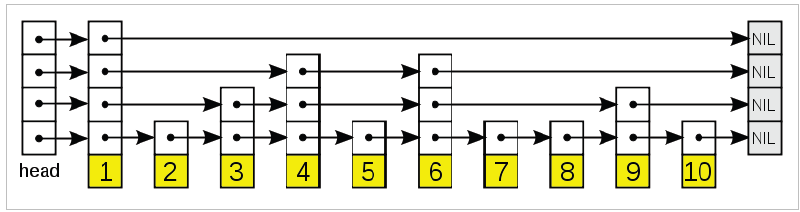
\includegraphics[scale=0.4]{assets/skip-list.png}
\end{center}

\paragraph{Theorem:}  
The expected tower height is $1$.

\paragraph{Proof:}
\[
\mathbb{E}[h] = \sum_{c=0}^{\infty} \frac{1}{2^{c+1}} = 1.
\]

\paragraph{Search algorithm:}

\begin{minted}[fontsize=\small, linenos]{python}
def find(x):
    v = head  # or -infinity in other definitions
    while v.height >= 0:
        if v.right <= x:
            v = v.right
        else:
            v = v.down
    return v
\end{minted}

\paragraph{Time complexity.}

We first bound the maximum tower height. Although unbounded in theory,
\[
\Pr[h \ge 2\log n] = \frac{1}{2^{2\log n}} = \frac{1}{n^2}.
\]
So the probability that *any* of the $n$ towers exceeds height $2\log n$ is $\frac{1}{n}$.

To simplify analysis, we rewrite the search algorithm from bottom to top:

\begin{minted}[fontsize=\small, linenos]{python}
def find(x):
    v = bottom_level_node(x)
    while v != head:   # or -infinity sentinel
        if v.has_up():
            v = v.up
        else:
            v = v.left
    return v
\end{minted}

This inverted version has the same time complexity.

We have
\[
\Pr[v.\text{has\_up}] = \frac{1}{2}.
\]
To climb to height $2\log n$, the expected number of attempts is
\[
2 \cdot 2\log n = O(\log n).
\]

\section{Game Tree Evaluation}
\begin{center}
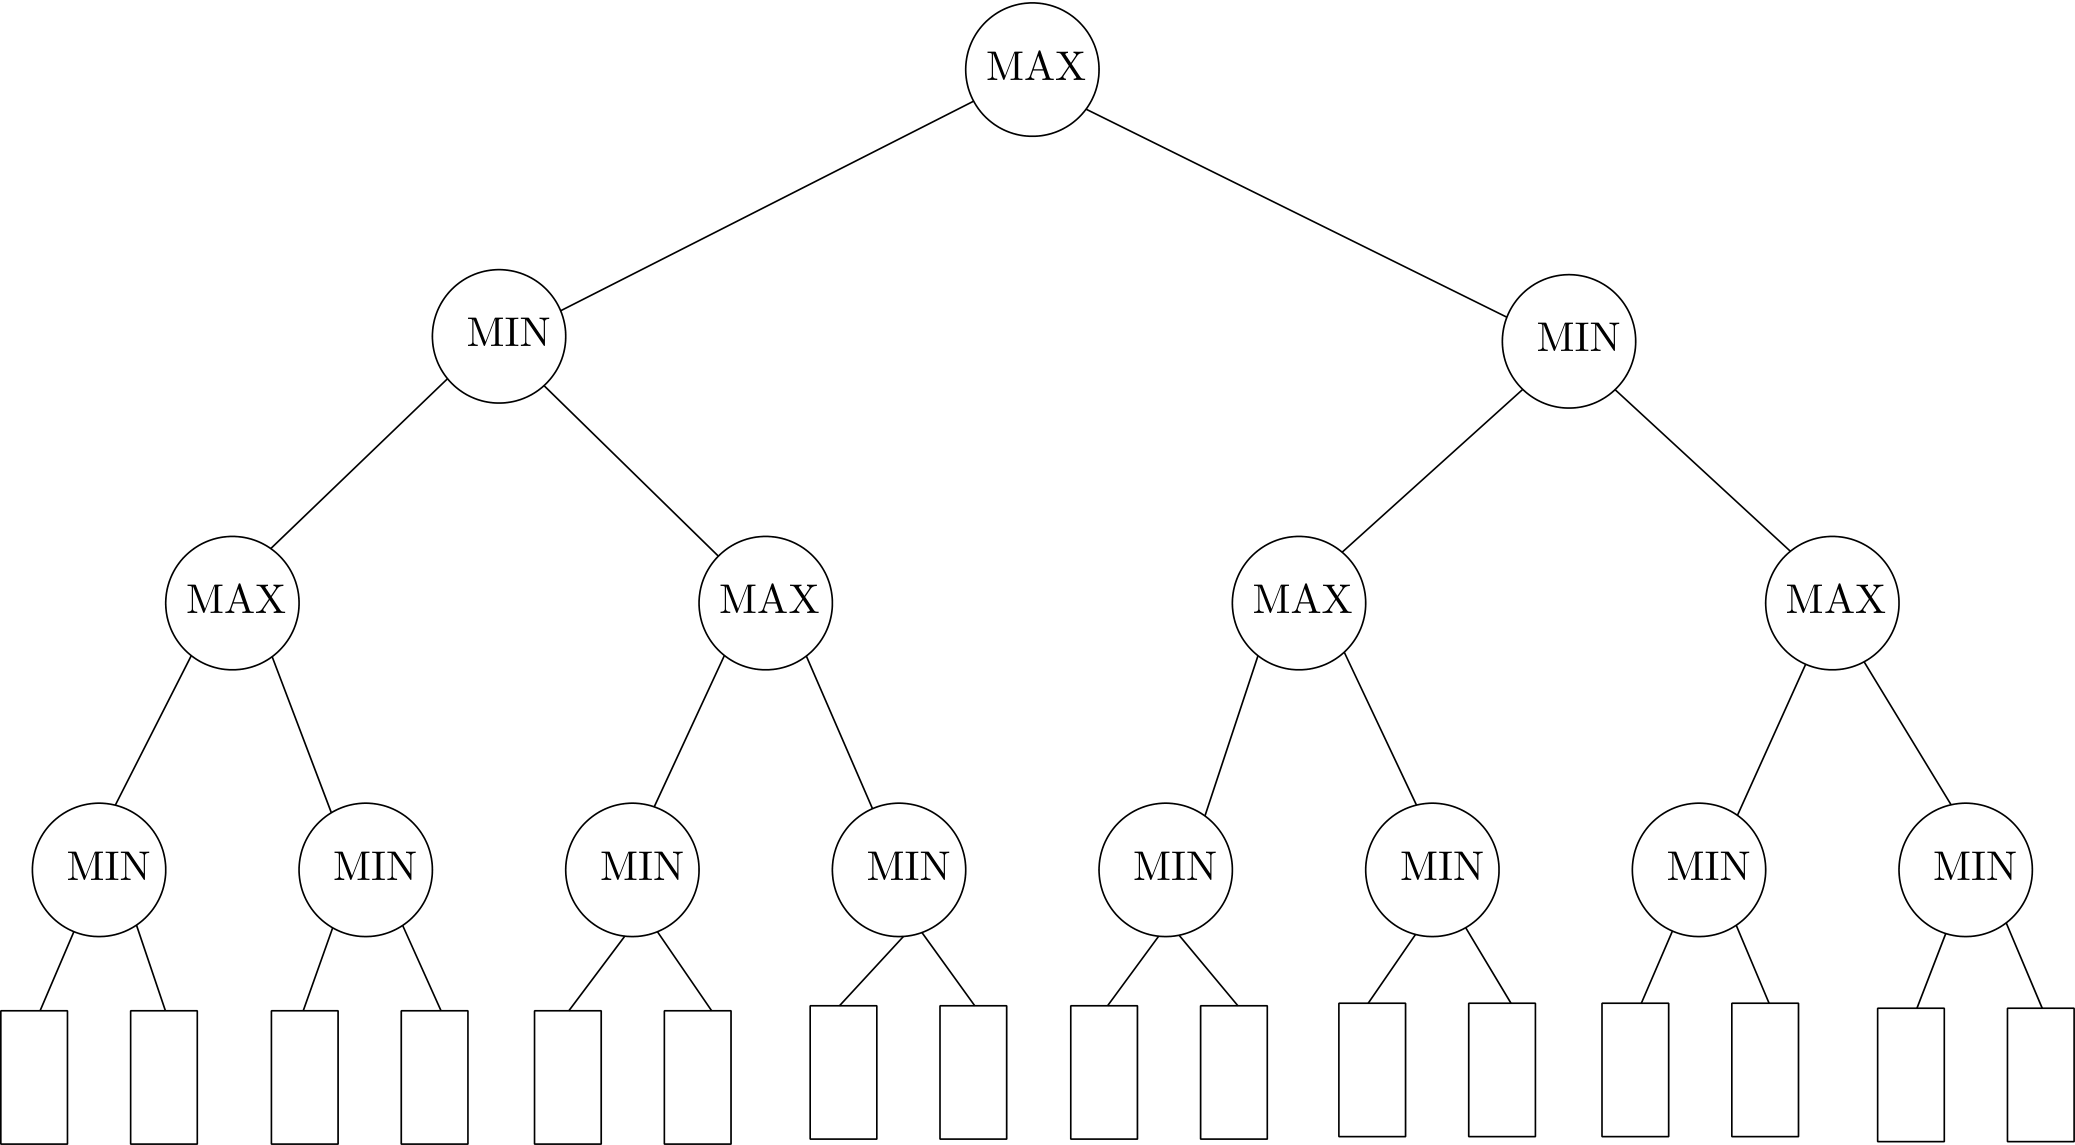
\includegraphics[scale=0.7]{assets/GameTreeEx.png}
\end{center}

We evaluate the value of the root of a full binary game tree.  
Given $k$ alternations between max- and min-nodes, the depth is $d = 2k$.

A naive DFS has time complexity
\[
O(2^d) = O(4^k).
\]

A randomized algorithm reduces this to $3^k$.

\subsection{Randomized Algorithm}

\paragraph{Idea:}
If a max-node ever evaluates to $1$, we know at least one child is $1$, so we can skip evaluating the other child.  
This happens with probability $1/2$.

Similarly, if a min-node evaluates to $0$, both children are $0$, so one subtree can be skipped.

\paragraph{Algorithm:}

\begin{minted}[fontsize=\small, linenos]{python}
def EVAL(v):
    i = rand(0, 1)
    r_i = EVAL(v[i])   # i = left or right child
    if (r_i == 1 and v.is_max) or (r_i == 0 and v.is_min):
        return r_i
    else:
        return EVAL(v[1 - i])
\end{minted}

\paragraph{Time Complexity:}
We show $E_k = O(3^k)$ by induction.

\begin{proof}
Base case $k=0$ is trivial: $E_0 = O(1) = O(3^0)$.

Inductive step: Assume $E_{k-1} = O(3^{k-1})$.

There are two symmetric cases:

\begin{itemize}
    \item If $\mathrm{EVAL}(v)=1$:
    \[
    E_k = 2E_{k-1} + \frac{1}{2} \cdot 2E_{k-1} = 3E_{k-1}.
    \]
    \item If $\mathrm{EVAL}(v)=0$:
    \[
    E_k = \left(E_{k-1} + \frac{1}{2} E_{k-1}\right) \cdot 2 = 3E_{k-1}.
    \]
\end{itemize}

Thus in all cases:
\[
E_k = 3E_{k-1} = O(3^k).
\]
\end{proof}

\section{Amortized Analysis}

\textbf{Until now:} Analysis of algorithms was done based on worst-case or expected time complexity.

\begin{itemize}
    \item Heap-Sort: $O(n \log n)$ worst case
    \item Skiplist: $O(\log n)$ expected
\end{itemize}

We want to tighten those bounds through some techniques.


\subsection{Introductory Example: Incremental Counter}

\begin{itemize}
    \item Represented through $k$ bits
    \item All set to zero at start
    \item Operations allowed: Increment the counter by one (usual $+1$ on an int)
\end{itemize}

We define the cost of an increment as the number of bit flips.

\medskip
\noindent
\textbf{Example:} $00011011 \xrightarrow{+1} 00011100$ causes three bit flips.

\medskip
\noindent
\textbf{Worst-Case:} The worst case is $011\ldots111$; an increment will cost $\Theta(k)$.

So for all increments ($2^k - 1$ possibilities), we can make a rather crude bound of $(2^k - 1) \cdot k$.

However, we can look a bit deeper and realize:

\begin{itemize}
    \item The last bit flips every time
    \item The second-to-last bit flips every two times
    \item The third-to-last bit flips every four times
    \item And so on
\end{itemize}

So for bit $i$ (starting from behind), it switches every $2^i$ times.

We can notice that this resembles a geometric series.

\medskip
\noindent
\textbf{Amount of flips from $0$ to $2^k - 1$:}
\[
(2^k - 1) \cdot \sum_{i=0}^{k} \frac{1}{2^i} 
\leq (2^k - 1) \cdot \sum_{i=0}^{\infty} \frac{1}{2^i} 
= (2^k - 1) \cdot 2
\]

\textbf{Note:} This argumentation is too specific for this data structure.

\medskip
\noindent
\textbf{Objective:} A more generalized framework for amortized analysis of a data structure for which a sequence of operations is executed.


\subsection{Generalized Framework}

Let $\Psi$ be the set of states of the data structure (in our example, it would be each bitset possibility).

We define the \emph{potential function} $\phi: \Psi \to \mathbb{N}_0$ that assigns to each state a natural number.

For an operation $\text{op}$ which transitions from $s_1 \in \Psi$ to $s_2 \in \Psi$ and has a real cost of $\text{rcost}(\text{op})$, we define:
\[
\text{acost}(\text{op}) := \text{rcost}(\text{op}) - \phi(s_1) + \phi(s_2)
\]


\paragraph{Theorem:} 
If we pick $\phi$ so that $\text{acost}(\text{op}) \in O(1)$, then the average real cost of a longer sequence is also $O(1)$.

\medskip
\noindent
\textbf{Note:} In our example, we can use $\phi(s) = $ number of 1s in $s$. This works because:

We can define $x$ as the number of consecutive 1s from the right. An operation causes $x + 1$ flips: all those ones turn to zero and one zero turns to one.

This means the number of 1s is reduced by $x - 1$. Therefore:
\[
\text{acost}(\text{op}) = (x + 1) - (x - 1) = 2 \in O(1)
\]

So we arrive at the same conclusion.


\paragraph{Proof of the Theorem:}
Consider a sequence of $l$ operations:

\[
\sum_{i=1}^{l} \text{acost}(\text{op}_i) 
= \sum_{i=1}^{l} \left( \text{rcost}(\text{op}_i) + \phi(s_{i+1}) - \phi(s_i) \right)
\]

When we analyze the sum, all the $\phi$ terms telescope and cancel except the first and last:
\[
= \sum_{i=1}^{l} \text{rcost}(\text{op}_i) + \phi(s_{l+1}) - \phi(s_1)
\]

Solving for the sum of real costs:
\[
\sum_{i=1}^{l} \text{rcost}(\text{op}_i) 
= \sum_{i=1}^{l} \text{acost}(\text{op}_i) - \phi(s_{l+1}) + \phi(s_1)
\]

Dividing by $l$ to get the average:
\[
\underbrace{\frac{\sum_{i=1}^{l} \text{rcost}(\text{op}_i)}{l}}_{\text{Average real cost}} 
= \frac{\sum_{i=1}^{l} \text{acost}(\text{op}_i) - \phi(s_{l+1}) + \phi(s_1)}{l}
\]

\[
= \frac{O(l) - \phi(s_{l+1}) + \phi(s_1)}{l} 
= O(1) + \frac{-\phi(s_{l+1}) + \phi(s_1)}{l}
\]

As $l \to \infty$, the term $\frac{-\phi(s_{l+1}) + \phi(s_1)}{l} \to 0$, confirming that the average real cost is $O(1)$.
\subsection{2--4 Trees}

These trees are not the same as those seen in the DSA seminar; they follow a different structure.

\begin{itemize}
    \item All leaves have the same depth.
    \item All keys appear in the leaves (ordered from left to right).
    \item All inner nodes contain 1, 2, or 3 keys and have 2, 3, or 4 children respectively.
    \item All keys appear twice inside the tree, except for the largest one.
\end{itemize}

\subsubsection{Example}

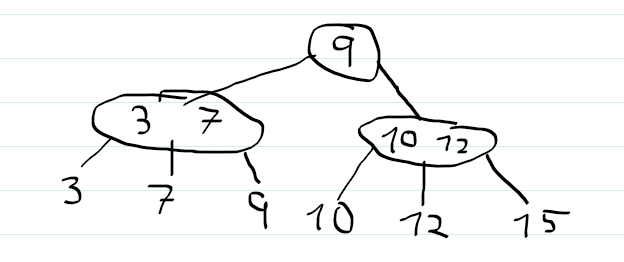
\includegraphics[scale=0.8]{assets/23tree.png}

\subsubsection{Extra Info}

For a tree of height $h$ with $n$ leaves,
\[
2^h \leq n \leq 4^h 
\quad \Rightarrow \quad 
\frac{1}{2}\log_2 n \leq h \leq \log_2 n
\]

This means that we can find any key inside the tree in $O(\log n)$ time.

\subsubsection{Insertion into the Tree}

\begin{enumerate}
    \item Find the element inside the tree (or its desired position).
    \item Attach the new leaf to its parent node.
\end{enumerate}

\paragraph{Possible Issue:}
The parent node may already be full, and attaching a new leaf can cause it to \emph{overflow}, reaching 5 children.

\paragraph{Solution:}
Split the parent node into two nodes and reassign the children accordingly.  
This splitting can propagate upwards, as the same issue may occur in ancestor nodes.

In the worst case, a single insertion can therefore take up to $O(\log n)$ time.

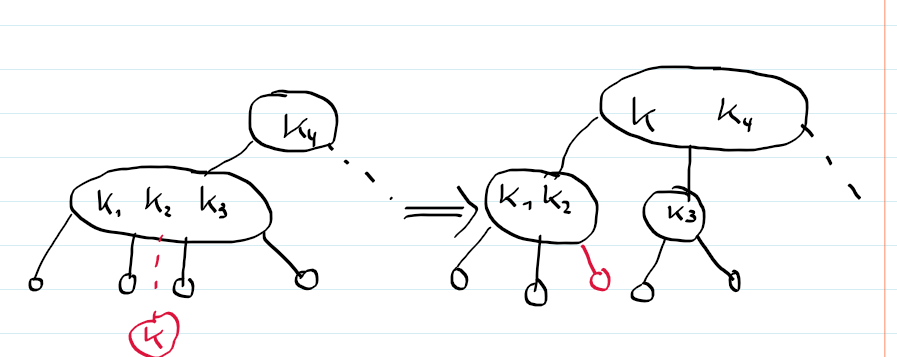
\includegraphics[scale=0.6]{assets/split.png}

\paragraph{Note:}
Instead of splitting and propagating, it is sometimes possible to send one of the extra children to a sibling node (only if the sibling has fewer than 4 children).  
We will not use this technique.

\subsubsection{Deletion from the Tree}

Deletion follows a similar approach. However, after deletion, a node may end up with only one child, which is not allowed.  
This is resolved using \textbf{melting} of nodes.

As with insertion, this issue can propagate upwards and take up to $O(\log n)$ time.

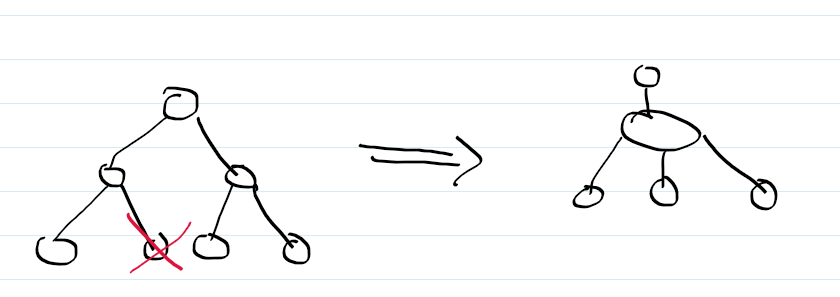
\includegraphics[scale=0.6]{assets/melt.png}

\paragraph{Note:}
Alternatively, we could use \emph{stealing} from a sibling node if the sibling has more than 2 children.

\subsubsection{Goal}

Our goal is to prove that for an arbitrary sequence of insertions and deletions, the \emph{average cost} is $O(1)$.

We will use amortized analysis. To do so, we define a potential function that represents how close the structure is to a “bad event.”

In the bit-flip example, the potential was the number of 1s. A high potential implied an inevitable expensive operation.

The potential function we choose is:
\[
\begin{aligned}
&\phi(t) := 0 \cdot \text{Number of nodes with 3 children} \\
&+ 1 \cdot \text{Number of nodes with 2 children} \\
&+ 2 \cdot \text{Number of nodes with 4 children} \\
&+ 2 \cdot \text{Number of nodes with 1 child} \\
&+ 4 \cdot \text{Number of nodes with 5 children}
\end{aligned}
\]


(5 children means a node that had 4 children and received an insertion.  
Similarly for nodes with 1 child.)

Nodes with 3 children are stable: neither insertion nor deletion propagates.  
Nodes with 2 or 1 child are dangerous for deletion, while nodes with 4 or 5 children are dangerous for insertion.

\paragraph{Statement:}
The amortized cost of a split or a melt is $\leq 0$.

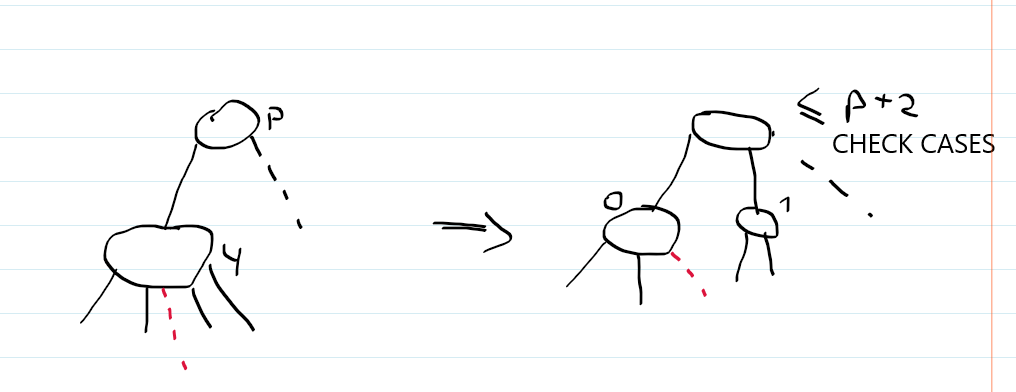
\includegraphics[scale=0.5]{assets/splitexample.png}

\[
\Rightarrow \text{acost(split)} \leq 1 + (p + 3) - (p + 4) = 0
\]

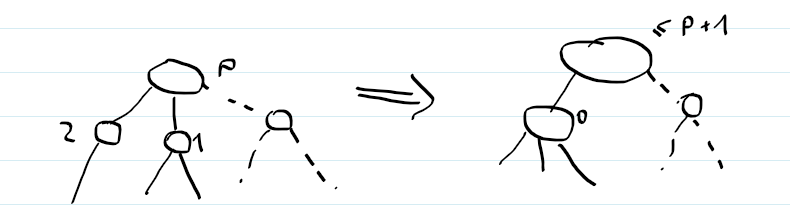
\includegraphics[scale=0.6]{assets/meltexample.png}



\[
\Rightarrow \text{acost(melt)} = 1 + p + 1 - (p - 3) = -1 \leq 0
\]

\paragraph{Note:}
This explanation is valid only for this specific configuration.  
For other configurations, we could instead steal a child from a sibling node.

In general:
\begin{itemize}
    \item Insertion increases the potential by at most 2.
    \item Deletion increases the potential by at most 1.
\end{itemize}

Thus, excluding the localization cost, the total amortized cost of insertion is
\[
\underbrace{O(1)}_{\text{attaching the leaf}} 
+ 
\underbrace{x \cdot (\leq 0)}_{\text{possible propagation}} 
= O(1)
\]

Deletion follows analogously.

\subsubsection{Uses of (2--4) Trees}

\paragraph{Use 1: Sorting Previously Sorted Sequences}

\subparagraph{Setup}
Given a sequence $x_1, x_2, \ldots, x_n$, define the number of inversions as
\[
  F := \left|\{(i,j) : i < j \text{ and } x_i > x_j\}\right|
\]
For a completely reversed array,
\[
  F = \frac{n(n-1)}{2}
  \quad \text{and} \quad
  0 \leq F \leq \frac{n(n-1)}{2}
\]

\subparagraph{Main Result}
Using (2--4) trees with repeated insertion, we achieve sorting time complexity of
\[
  O\left(n + n \log\left(\max\left(1, \frac{F}{n}\right)\right)\right)
\]
For partially sorted arrays, this provides a significant improvement over standard sorting algorithms. In the worst case, it still runs in $O(n \log n)$ time.

\subparagraph{Algorithm}
Rather than localizing each insertion from the root, we start from the rightmost leaf and walk upward until finding the appropriate subtree, then search downward.

\vspace{0.5em}
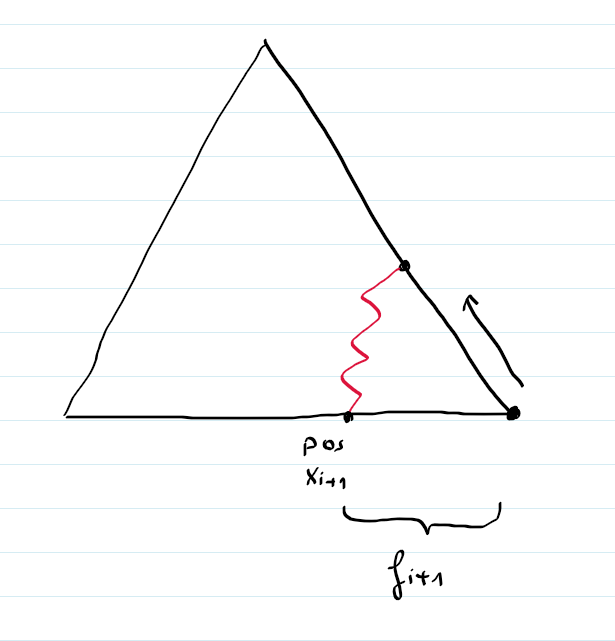
\includegraphics[scale=0.5]{assets/24tree.png}

\subparagraph{Key Observation}
Define $f_{i+1} = \left|\{j : j < i + 1 \text{ and } x_j > x_{i+1}\}\right|$ as the number of elements already in the tree that should appear to the right of $x_{i+1}$.

\subparagraph{Localization Cost}
$x_{i+1}$ can be localized in $O(1 + \log(\max(1, f_{i+1})))$ time complexity.

\subparagraph{Proof}
The algorithm traverses upward from the rightmost leaf until reaching a node $v$ where $x_{i+1} >$ rightmost key of $v$. Then we proceed with the usual downward search.

We have $f_{i+1} \geq \#\{\text{leaves under } v''\}$ (where $v''$ is a sub-sub-child of $v$). 
This implies $v'' \geq 2^{h-2}$ if we take $h$ steps upward.

Therefore,
\[
  h \leq 2 + \log(f_{i+1})
\]

The total time complexity for localizing all insertions is:
\begin{align*}
  &\sum_{i=1}^{n-1} \left(1 + \log(\max(1, f_{i+1}))\right) \\
  &= O\left(n + \sum_{i=1}^{n-1} \log(\max(1, f_{i+1}))\right)
\end{align*}

Since $\sum_{i=1}^{n-1} f_{i+1} = F$, the worst case for $\sum \log f_{i+1}$ occurs when all $f_{i+1}$ are equally distributed (by concavity of logarithm), giving each $f_{i+1} = \frac{F}{n}$. Thus:
\[
  O\left(n + n \log\left(\frac{n + F}{n}\right)\right) = O\left(n + n \log\left(\max\left(1, \frac{F}{n}\right)\right)\right)
\]

\paragraph{Use 2: Efficient Mixing via Finger Search}

\subparagraph{Concept: Finger Search}
Finger search starts the search at the position of a recently inserted node rather than from the root, enabling faster localization when the target is close to the finger.

\subparagraph{Problem}
Naively merging two (2--4) trees by repeatedly popping from one and inserting into the other takes $O(n \log n)$ time. Naive finger search can perform poorly since two nearby nodes may only be connected through the root.

\subparagraph{Solution: Level-Connected Trees}
We augment (2--4) trees with level connections, linking siblings at each level.

\vspace{0.5em}
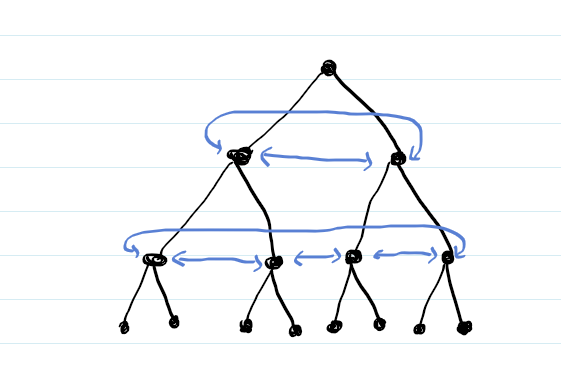
\includegraphics[scale=0.5]{assets/levelconnectedtree.png}

\subparagraph{Finger Search Lemma}
In a level-connected (2--4) tree, finger search takes time complexity
\[
  O(\log(\min(d, n - d)))
\]
where $d$ is the distance (measured in leaves) between the finger position and the destination.

\subparagraph{Proof of Lemma}
To search for $x$:
\begin{enumerate}
  \item Traverse upward from the finger until reaching node $v$ such that either $v$, $v.\text{rightneighbor}$, or $v.\text{leftneighbor}$ contains $x$ in its subtree.
  \item Execute the usual downward search.
\end{enumerate}

The time complexity is bounded by the height of $v$, which is $O(\log(\min(d, n - d)))$.

\subparagraph{Efficient Merging Algorithm}
To merge two level-connected (2--4) trees $B_1$ and $B_2$:
\begin{enumerate}
  \item Start finger search from the leftmost leaf of $B_1$ at the position of its last inserted element.
  \item Insert elements of $B_2$ in increasing order.
\end{enumerate}

Let $B_1 = \{\overline{x}_1, \overline{x}_2, \ldots, \overline{x}_n\}$ and $B_2 = \{\underline{x}_1, \underline{x}_2, \ldots, \underline{x}_m\}$.

Define $d_i$ as the distance (in leaves) from the position of $\underline{x}_i$ in $B_1$ to the position of $\underline{x}_{i-1}$ in $B_1$. 

Since $\sum_{i=1}^{m} d_i \leq n$ (at most $n$ original leaves), the search cost for $x_i$ is $O(1 + \log(1 + d_i))$.

\subparagraph{Total Merge Cost}
The total cost is:
\begin{align*}
  &\sum_{i=1}^{m} (1 + \log(1 + d_i)) \\
  &\leq m + \sum_{i=1}^{m} \log\left(1 + \frac{n}{m}\right) \\
  &= m + m \log\left(\frac{m + n}{m}\right) \\
  &\leq 2m \log\left(\frac{m + n}{m}\right) \\
  &= 2 \log\left(\left(\frac{m + n}{m}\right)^m\right) \\
  &\leq 2 \log\left(\binom{m+n}{m}\right)
\end{align*}

Therefore, we can merge two (2--4) trees in $O\left(\log\left(\binom{m+n}{m}\right)\right)$ time complexity.

\subparagraph{Remark on Balance Insensitivity}
For two trees of sizes $n_1$ and $n_2$ with $n_1 + n_2 = n$, the merge time is
\[
  \log\left(\binom{n_1+n_2}{n_2}\right) = \log(n!) - \log(n_1!) - \log(n_2!)
\]

Interestingly, the balance of the tree sizes does not significantly affect the time complexity. This contrasts with merge sort, where symmetric partitions are essential for optimal performance.


\section{Linear Programming}
\subsection{Introductory Example}
For a human to keep a balanced diet, he must eat
\begin{itemize}
    \item At least 11 unit of Carbohydrates
    \item At least 7 units of protein
    \item At least 5 units of fat
\end{itemize}

The consumer can buy the following items
\begin{align}
    \begin{tabular}{|c|c|c|c|c|}
        \hline
        Item & Carbohydrates & Protein & Fats & Price\\
        \hline
        Meat & 1 & 3 & 5 & 7 Euro\\
        \hline
        Tofu & 2 & 2 & 0  & 3 Euro\\
        \hline
        Bread & 4 & 1 & 0  & 2 Euro\\
        \hline
        Cheese & 1 & 4 & 2  & 4 Euro\\
        \hline
    \end{tabular}
\end{align}

Objective: Meet the health requirements while minimizing cost

\subsubsection{Problem solving strategies}

We know
\[x_m \geq 0 \text{ Meat}\]
\[x_t \geq 0 \text{ Tofu}\]
\[x_b \geq 0 \text{ Bread}\]
\[x_c \geq 0 \text{ Cheese}\]


\paragraph{Linear Programm: }
\[\text{Price: } 7x_m + 3x_t + 2x_b + 4x_c \text{ Output we want to minimize}\]
\[\text{Carbohydrates: } 1x_m + 2x_t + 4x_b + 1x_c \geq 11\]
\[\text{Protein: } 3x_m + 2x_t + 1x_b + 4x_c \geq 7\]
\[\text{Fats: } 5x_m + 0x_t + 0x_b + 2x_c \geq 5\]



\textbf{Linear Programms (LPs)} can model so many different problems such as
\begin{itemize}
    \item Max Flow, min cut
    \item Minimum enclosing annulus
    \item Shortest Path
\end{itemize}


\subsection{Geometrical Interpretation for LPs}
Using another easier example.

\[max(x+y)\]
\[y \geq -x+3\]
\[y \leq -0.5x+7\]
\[y \geq 0.5x\]
\[y \leq 0.5x+3\]


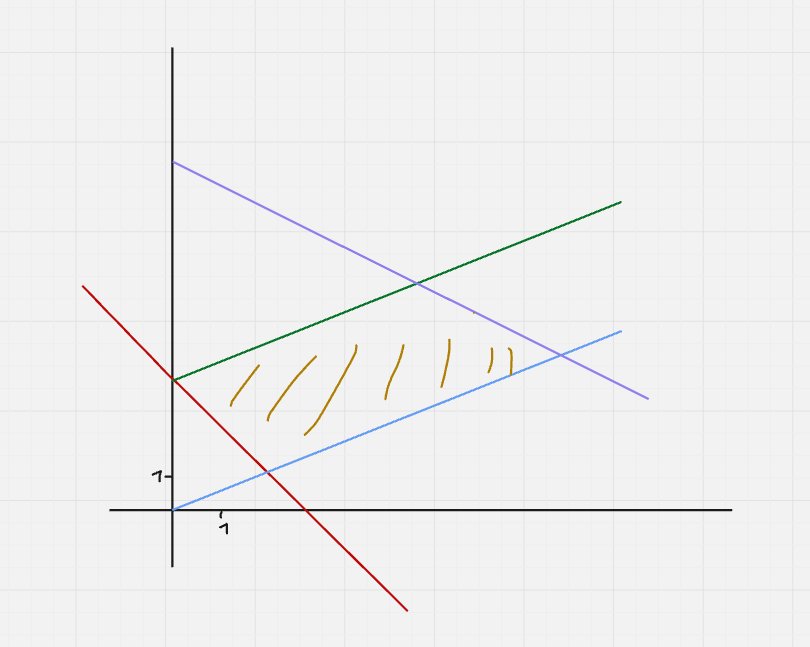
\includegraphics[scale=0.5]{assets/LPs.png}

In this case is the Zufälligkeitsbereich convex, which means, for linear end function, the optimum will be found at one of the corners.

The rough approach would be start at ZiFu = 0 (which translates to the line $y=-x$, and move the function upwards/sideways, until we find the last point that still crosses with the function thats within our Polygon)

\subsection{Naiv Solving Strategies}
Compute the Halbraumsschnitt and check all its corners

For two dimensions its OK, but grows exponentially for higher dimensions $n^{\lfloor \frac{d}{2}\rfloor}$

Where d:= Nº Dimensions and n:= Nº Constraints

\subsection{(Commercial) Solvers for LPs}
\begin{itemize}
    \item CPLEX - uses glpk
    \item GUROBI - Lpsolver
\end{itemize}

\subsection{Algorithms to solve LPs}
\begin{itemize}
    \item Simplex: Practically, amazing but there are some rare theoretical scenarios where it struggles
    \item Ellipsical Method: Theoretically good, but practically unusable
    \item Interior Point Methode: Theoretically and practically good.
\end{itemize}

\textbf{Our Algorithm:} We will design an algorithm that for a fix d runs in $O(n)$
\[\text{Note: Time complexity is actually } O(2^{2^d} \cdot n)\]

\subsubsection{Prune and Search for LPs}
Idea: Pruning some of the constraints that dont mark the corners for the optimum

High-Level idea: On a round basis, throw away a constant amount of constraints that dont define the optimum

We have to accept some sacrifices for the rough idea
\begin{itemize}
    \item LP is in $\mathbb{R}^2$
    \item Objective: Lowest point in the Zufälligkeitsbereich. (min(y))
    \item There exists an optimum
\end{itemize}

\paragraph{How can we prune constraints? } We can divide the constraints $H$ into $H_{up}$ and $H_{down}$. depending on if they 'face' up or down

If we know that the optimum lies either on the left or right of a vertical line (see image below), given a pair $h_1,h_2 \in H_{up}$ we can prune as follows.

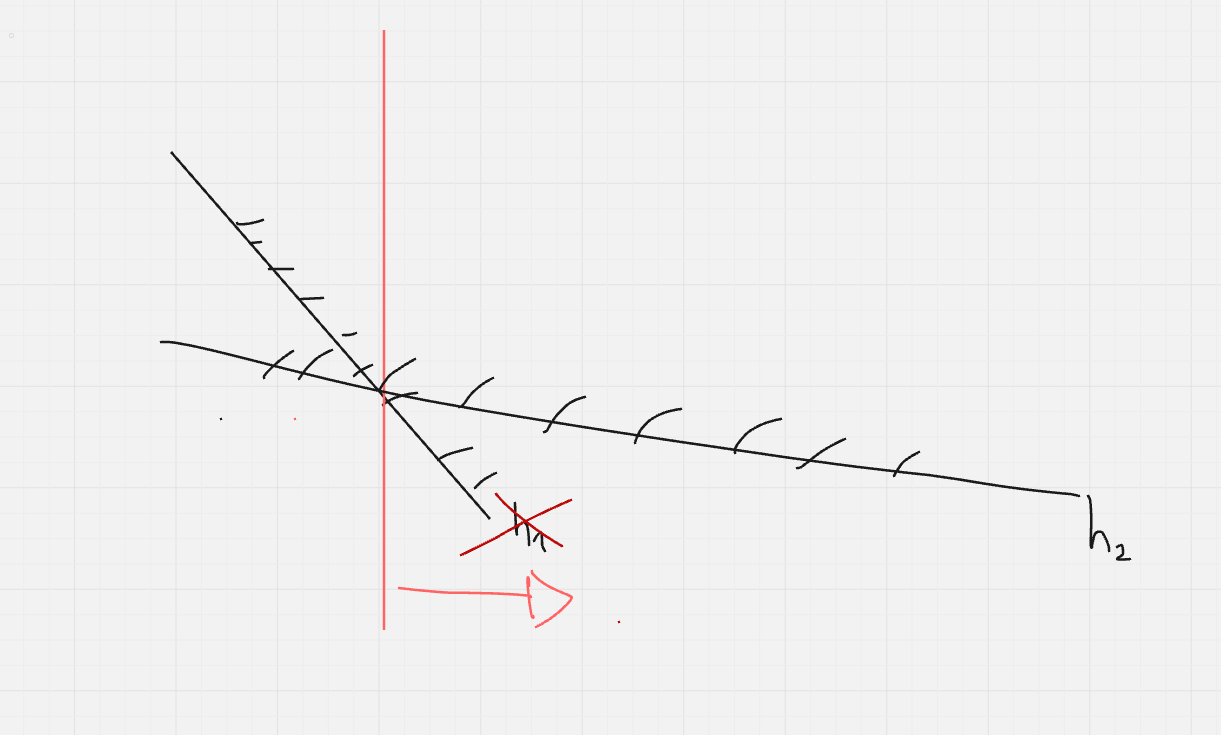
\includegraphics[scale=0.4]{assets/lsp2.png}


We can prune $h_1$ in this case, because the polygon is convex, and the objective is the lowest point, so will always be able to prune one of the two (analogously for $H_{down}$ pairs)


So what we do is we draw a vertical line in a set position (which will be determined later), and we determine two constraints

\begin{itemize}
    \item $P_{up}$, which is the $h \in H_{up}$ with the lowest y value
    \item $P_{down}$, which is the $h \in H_{down}$ with the lowest y value
\end{itemize}

We have two different possibilities (drawn below).

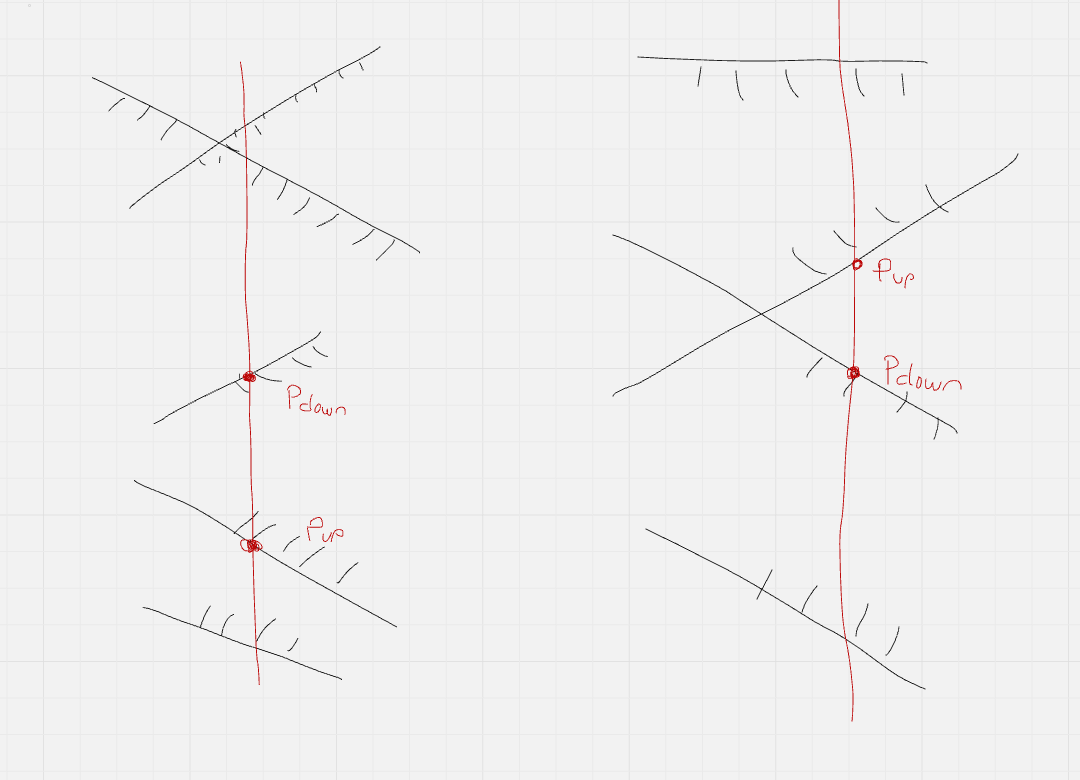
\includegraphics[scale=0.4]{assets/lps3.png}

\begin{itemize}
    \item $P_{up} < P_{down}$. This is the left case, we must go right (in this disposition) to find a lowest possible point
    \item $P_{up} > P_{down}$. This is the case on the right, to find the Zufälligkeitsbereich we MUST go left (in this disposition), so the direction is left.
\end{itemize}



So we have gotten to the conclusion that we can run one of these Oracle operations in $O(n)$, so to make the prune

\paragraph{Naive pruning: } Do this oracle operation for all   Pairs
\[\frac{n}{2} \text{ pairs } \cdot n = O(n^2)\]


\paragraph{Better pruning: } Build the pairs, compute the x-median of all those intersection points and draw the line there. We will be able to prune half of those intersections, which equates to removing $\frac{n}{4}$ constraints. We are left with $\frac{3n}{4}$If we repeat this process

\[ n + \frac{3n}{4} + \frac{9n}{16} + ... \leq 4n \in O(n)\]
\subsubsection{Prune and Search in $\mathbb{R}^3$}

\paragraph{Key Geometric Insight:}
When two constraint planes in $\mathbb{R}^3$ intersect, they form a line. If we construct a vertical plane containing this intersection line, knowing which side of the plane contains the optimal solution tells us which constraint can be safely discarded.

\textbf{IMPORTANT SIMPLICITY: All planes are 'pointed' upwards}
\paragraph{The Oracle (2D Prune and Search):}

To determine which side of the vertical plane contains the optimum, we use a 2D oracle:

\begin{enumerate}
    \item \textbf{Slice the 3D problem:} Take a 2D horizontal plane cutting through the 3D space
    \item \textbf{Reduce to 2D:} The intersection of all constraint planes with our horizontal plane produces a set of lines in that 2D plane
    \item \textbf{Find the optimum in 2D:} Execute a 2D prune-and-search algorithm to find the lowest point in this 2D slice
    \item \textbf{Extract directional information:} The lowest point lies on the intersection of two constraint lines. The direction of this intersection tells us which side of our vertical plane to keep and which constraint to discard
\end{enumerate}
\paragraph{Efficient Implementation:}

To use the oracle efficiently, we need to structure our problem carefully:

\begin{enumerate}
    \item \textbf{Pair the constraints:} Group the $n$ constraints into $\frac{n}{2}$ pairs. Each pair of planes intersects to form a line in 3D space
    
    \item \textbf{Project from above:} View these intersection lines from directly above (project onto the ground plane). Each projected line has a slope
    
    \item \textbf{Rotate for balance:} Rotate the viewing angle so that exactly half of the projected lines have positive slope ($>0$) and half have negative slope ($<0$)
    
    \item \textbf{Strategic pairing:} Pair constraints such that each pair consists of one line with positive slope and one with negative slope. When viewed in the 2D projection, these pairs form X-shapes
    
    \item \textbf{Result:} The 2D plane now contains a collection of X-patterns, where each X represents a pair of constraints with opposite slopes. This balanced structure allows efficient pruning
\end{enumerate}

\paragraph{The Pruning Process:}

\begin{enumerate}
    \item \textbf{X-median split:} 
    \begin{itemize}
        \item Find the $x$-coordinate of the median X-center (where each X crosses)
        \item Draw a vertical line through this x-median
        \item Use 2D prune-and-search to determine whether the optimum lies to the \textit{left} or \textit{right} of this line
        \item Mark all X's whose centers lie on the discarded side
    \end{itemize}
    
    \item \textbf{Y-median split:}
    \begin{itemize}
        \item For the X's that were discarded in the x-median split, find the $y$-coordinate of their median center
        \item Draw a horizontal line through this y-median
        \item Use 2D prune-and-search to determine whether the optimum lies \textit{above} or \textit{below} this line
    \end{itemize}
    
    \item \textbf{Double-discarded X's - Constraint Removal:}
    
    For all the double discarded X's we know in which direction the optimum lies.

    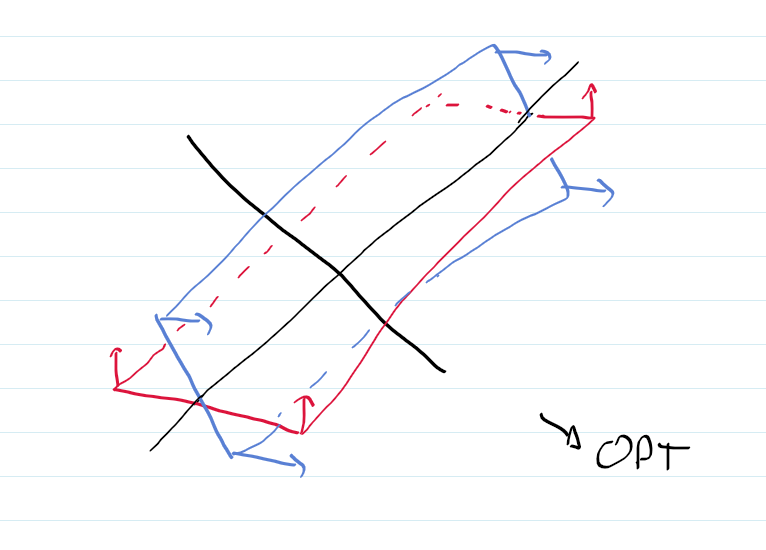
\includegraphics[scale=0.5]{assets/lpr3.png}
    
    Because the planes are pointed upwards, we can see that the red plane (in this case), deleting it wont affect the optimum.
\end{enumerate}

\paragraph{Analysis:}

So we have $n/2$ lines, that form $n/4$ X's, and for $n/16$ of them we can delete one of the constraints

So next iteration will have $15n/16$ constraints. Which is linear, but as we see, as dimensions rise it grows really exponentially


\textbf{CHECK NOTIZEN FOR CONSTRAINED SHORTEST PATH WITH PREFERENCE AND PARETO OPTIMIZATION}

\end{document} 
